\documentclass[../../main.tex]{subfiles}
\usepackage{fp}
\begin{document}
\chapter{Avatar Creation and Pose Synthesis}
\label{ch:avatar_creation_pose_synthesis}

Before we can animate \gls{sl}, a well-crafted avatar is essential. This chapter explores the avatar creation process and integrates rigging layers to the pre-existing low-level AZee synthesizer. Rigging, which sets up a skeletal structure to drive a character's mesh, is critical for achieving realistic movement and deformation, particularly in capturing the nuanced expressions of \gls{sl}.

A layered approach provides a sophisticated method for managing these complexities. By dividing the rigging process into distinct layers—each addressing specific aspects of movement and deformation—we gain greater control and flexibility. This strategy enables the synthesis system to function with multiple avatars and is faster and more accurate than the previous synthesizer.

In this chapter, section~\ref{ch:avatar_creation_pose_synthesis:proc_rig_signing_avatars} introduces a procedural rigging system for signing avatars, which automates the rigging process and enables the generation of complex \gls{sl} gestures. Section~\ref{ch:avatar_creation_pose_synthesis:results} presents the results of the implementation, and section~\ref{ch:avatar_creation_pose_synthesis:evaluation} evaluates the performance, accuracy, and quality of the animation. Finally, section~\ref{ch:avatar_creation_pose_synthesis:conclusion} concludes the chapter and discusses future work.

\section{Procedural Rigging for Signing Avatars}
\label{ch:avatar_creation_pose_synthesis:proc_rig_signing_avatars}

Rigs have been used in computer animation for decades to control the movement and deformation of characters. Traditional rigging systems typically consist of a hierarchical structure of bones, controllers, and constraints that define how the character’s mesh deforms in response to movement.

A signing avatar differs significantly from traditional systems. To begin with, no \gls{sl} uses the lower body in its articulation. This means that the rigging system for a signing avatar can be simplified to focus on the upper body as shown in figure~\ref{fig:upper_body_avatar}. 

\begin{figure}[h]
    \centering
    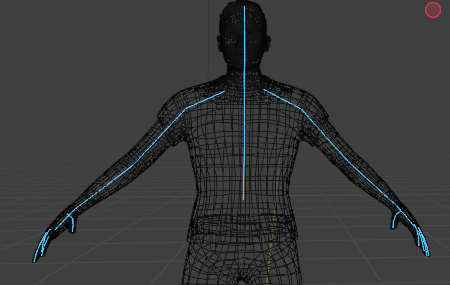
\includegraphics[width=0.5\textwidth]{chapters/avatar_creation_pose_synthesis/images/upper_body_avatar.png}
    \caption{An example of an upper body avatar rig}
    \label{fig:upper_body_avatar}
\end{figure}

However for procedurally animating a signing avatar, the complexity of \gls{sl} gestures and expressions poses unique challenges and necessitates a more sophisticated rigging system.

\subsection{AZee Blender interface}
\label{ch:avatar_creation_pose_synthesis:proc_rig_signing_avatars:azee_blender_interface}

The old synthesizer used a \emph{SkelSpec} structure (explained in section~\ref{ch:background_work:sign_language_synthesis:3d_techniques:sign_language_synthesis_systems:azee_based:low_level_synthesizer_for_azee:azee_blender_interface}) to sync an AZee posture and a blender armature. Due to the complexity of this \emph{SkelSpec} structure, the animation had too much latency. One of the first contributions of our work was to create a new interface for the low level synthesizer for AZee. This new interface didn't have a \emph{SkelSpec} (figure~\ref{fig:new_interface}) and interacted directly with the blender armature. 

\begin{figure}
    \centering
    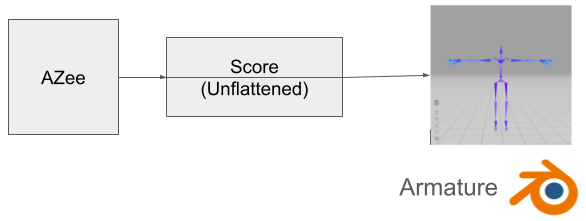
\includegraphics[width=0.5\textwidth]{chapters/avatar_creation_pose_synthesis/images/new_interface.png}
    \caption{The new interface of the low level synthesizer for AZee}
    \label{fig:new_interface}
\end{figure}

\subsection{Sites on the Avatar}
\label{ch:avatar_creation_pose_synthesis:proc_rig_signing_avatars:auto_site_generation}

The sites in the previous synthesizer were represented as blender empty objects and had to be manually created (explained in ~\ref{ch:background_work:sign_language_synthesis:3d_techniques:sign_language_synthesis_systems:azee_based:low_level_synthesizer_for_azee:azee_sites}) to automate this site creation, we can use AZee's bone structure as reference as it remains consistent across avatars. For this, we use \textbf{directional surface projection} (figure~\ref{fig:site_surface_projection}), where points are projected from a bone's position in a specified direction to detect intersections with the avatar's surface. In this case, the projection is initiated from a bone's position within the avatar's mesh, and the intersection point is used to generate a site. This algorithm generates sites based on the bone's location and orientation, ensuring that the sites are accurately positioned on the avatar's mesh. Algorithm~\ref{alg:site_generation_with_projection} outlines the projection process for automatic site generation.

\begin{figure}[ht]
    \centering
    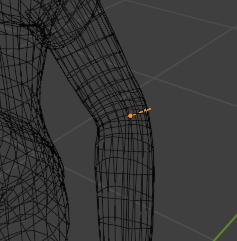
\includegraphics[width=0.5\textwidth]{chapters/avatar_creation_pose_synthesis/images/site_surface_projection.png}
    \caption{Projection example for left elbow site}
    \label{fig:site_surface_projection}
\end{figure}

\begin{algorithm}[ht]
    \caption{Projection Algorithm for Automatic Site Generation}
    \label{alg:site_generation_with_projection}
    \begin{algorithmic}
        \State \textbf{Input:} A 3D model with bones
        \State \textbf{Output:} Generated and positioned sites on the model

        \State $sites \gets$ an empty list to store generated site locations

        \State Remove existing sites from the model

        \State $armature \gets$ find the armature associated with the 3D model

        \For{each $bone$ in $armature$}
            \State $start\_point \gets$ determine the starting point based on the bone's position
            \State $direction \gets$ calculate the direction vector based on the bone's orientation
            
            \State $hit\_success, hit\_location \gets$ perform surface projection from $start\_point$ in $direction$
            \If{$hit\_success$}
                \State $site\_location \gets hit\_location$
            \Else
                \State $site\_location \gets$ fallback location based on predefined logic
            \EndIf

            \State Add $site\_location$ to the $sites$ list
            
            \State Apply any additional constraints or relationships between the site and the bone
        \EndFor

        \For{each $finger$ in the model}
            \For{each $segment$ in $finger$}
                \State Repeat the projection procedure to determine and store $site\_locations$ for each segment
            \EndFor
        \EndFor

        \State Finalize and store the $sites$ list for further processing or rendering
    \end{algorithmic}
\end{algorithm}

The generated sites can be visualized on the avatar in figure~\ref{fig:sites_bazeel_combined}.

\begin{figure}[h]
    \centering
    \begin{subfigure}[b]{0.3\textwidth}
        \centering
        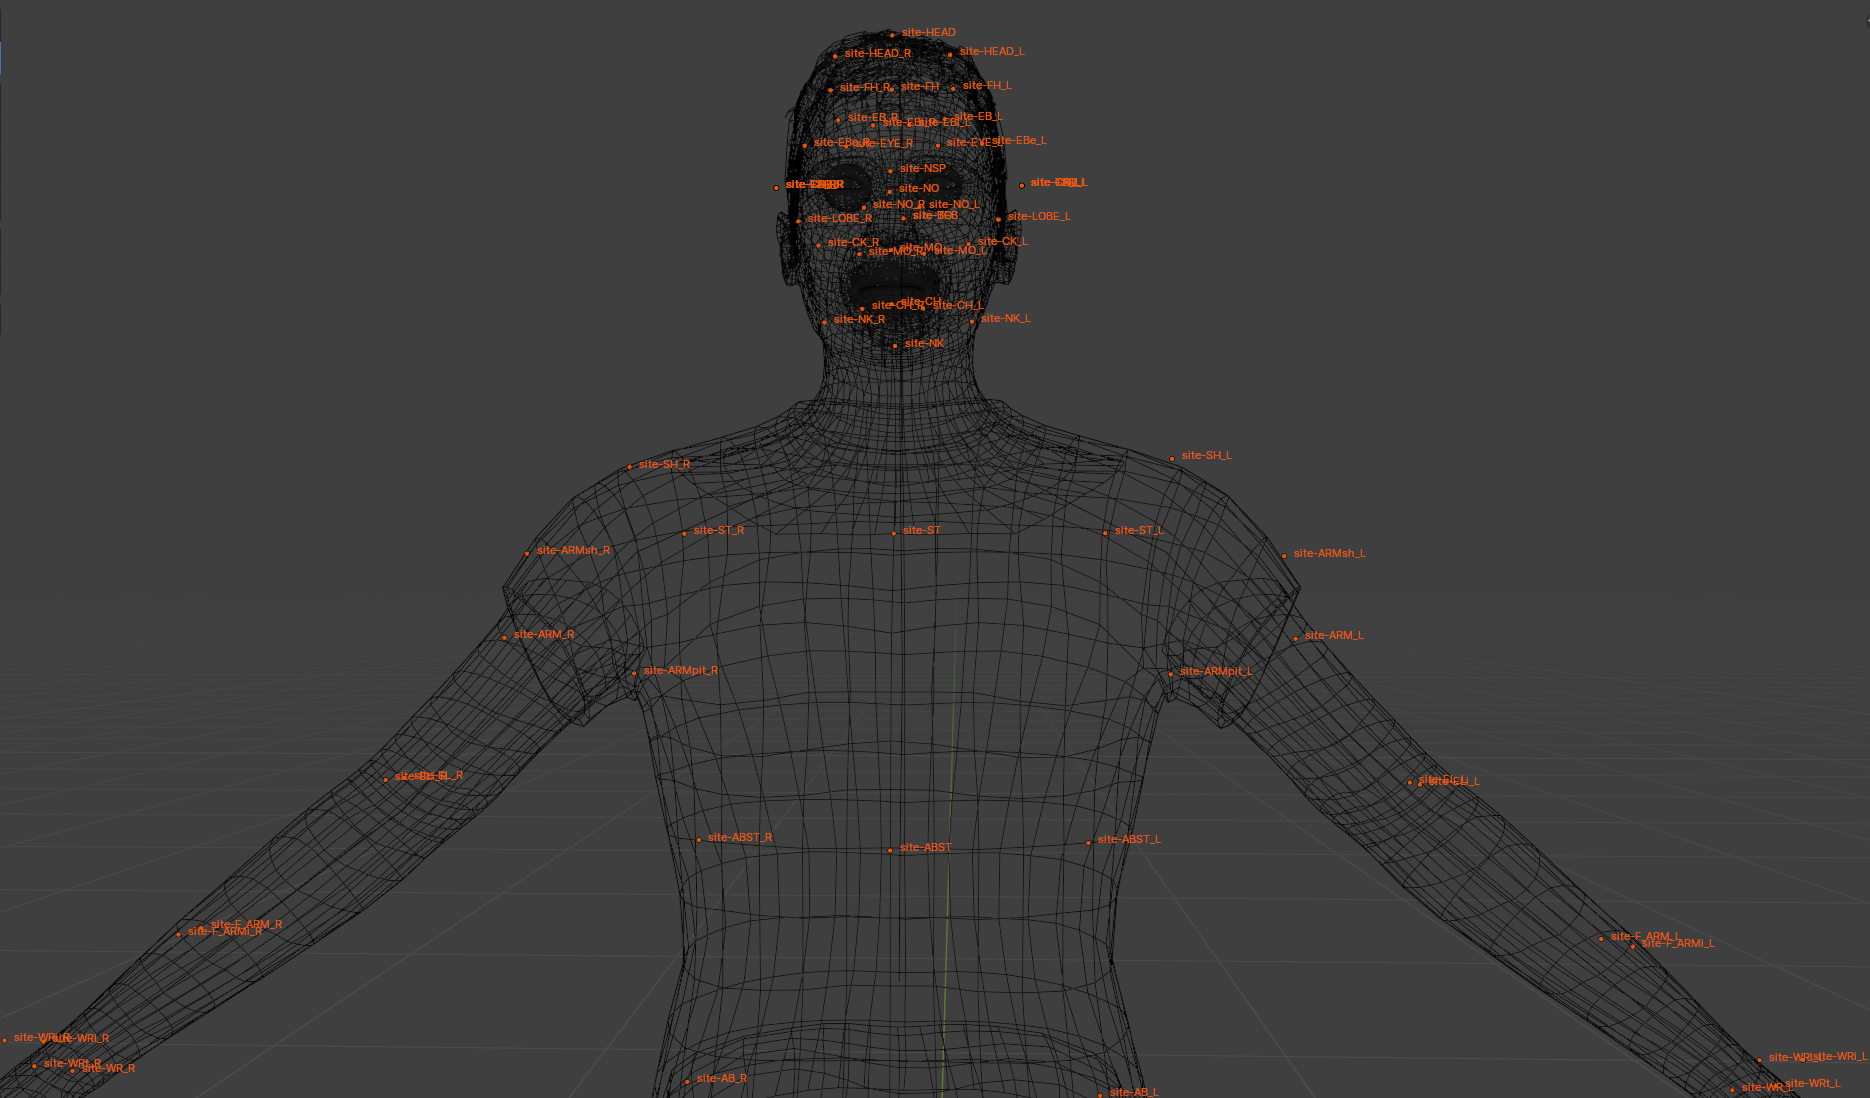
\includegraphics[width=\textwidth]{chapters/avatar_creation_pose_synthesis/images/sites_body_front.png}
        \caption{Front View of Body Sites}
        \label{fig:sites_body_front}
    \end{subfigure}
    \hfill
    \begin{subfigure}[b]{0.3\textwidth}
        \centering
        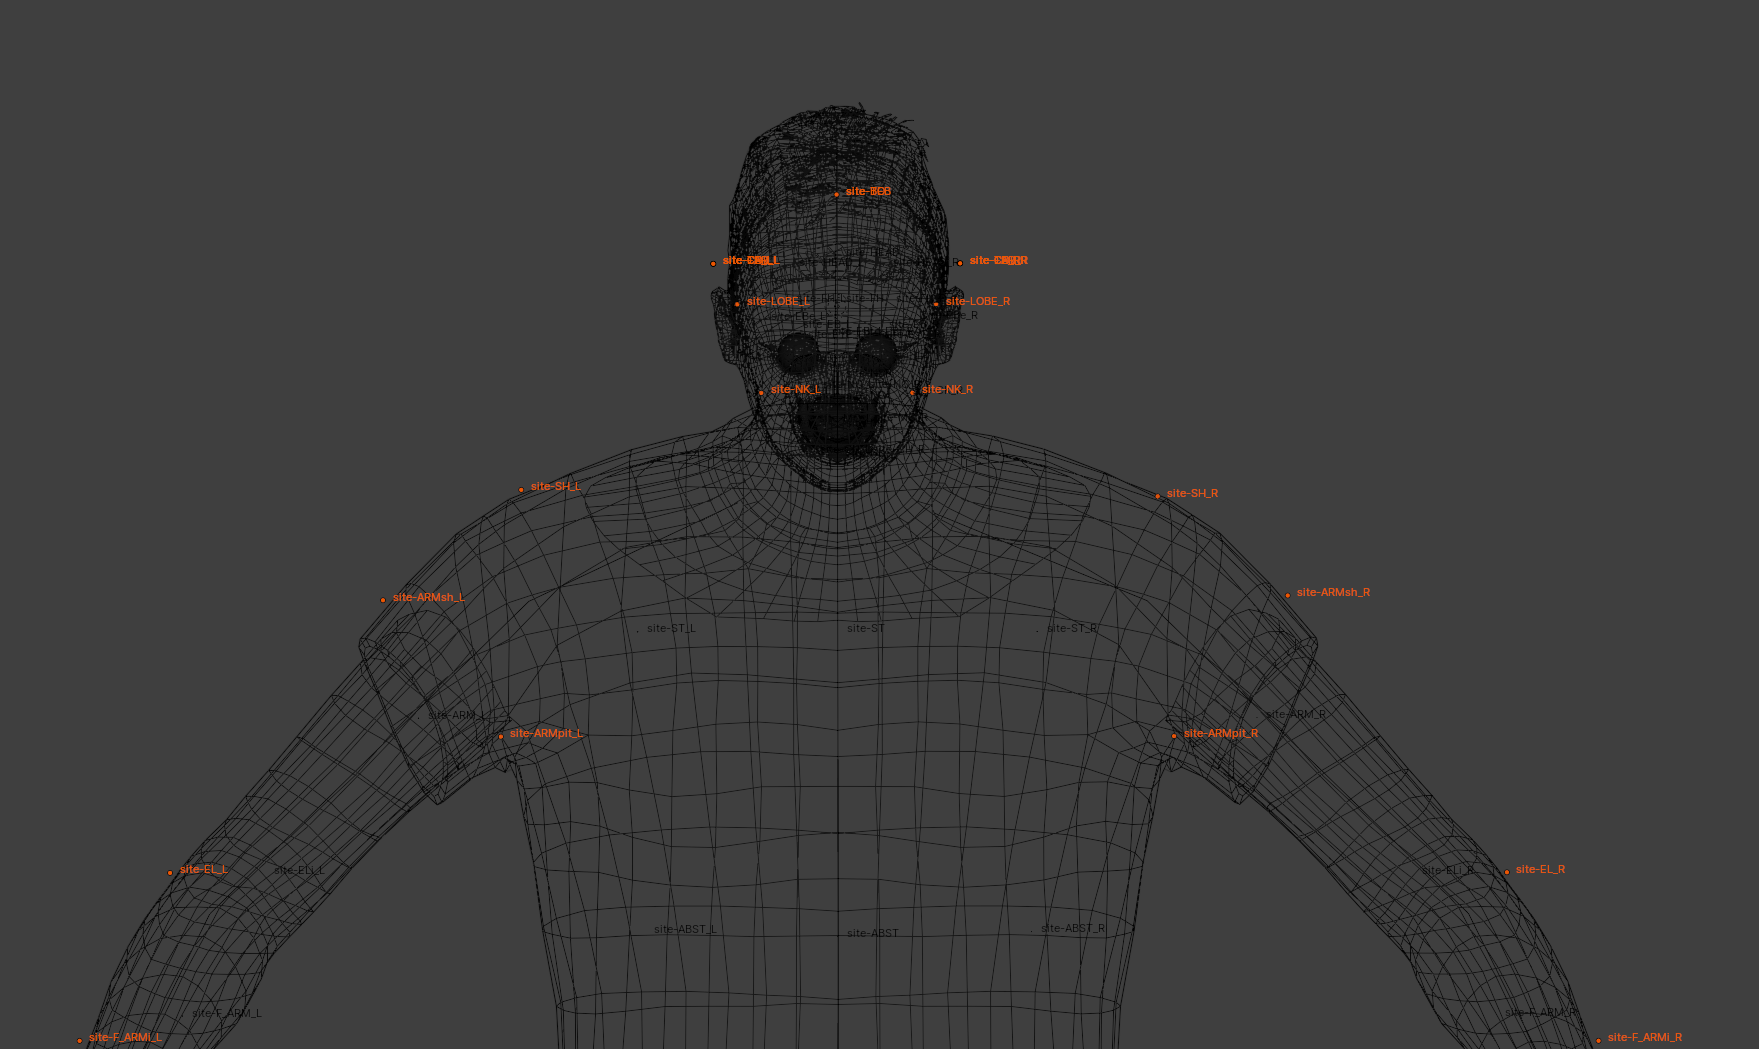
\includegraphics[width=\textwidth]{chapters/avatar_creation_pose_synthesis/images/sites_body_back.png}
        \caption{Back View of Body Sites}
        \label{fig:sites_body_back}
    \end{subfigure}
    \hfill
    \begin{subfigure}[b]{0.3\textwidth}
        \centering
        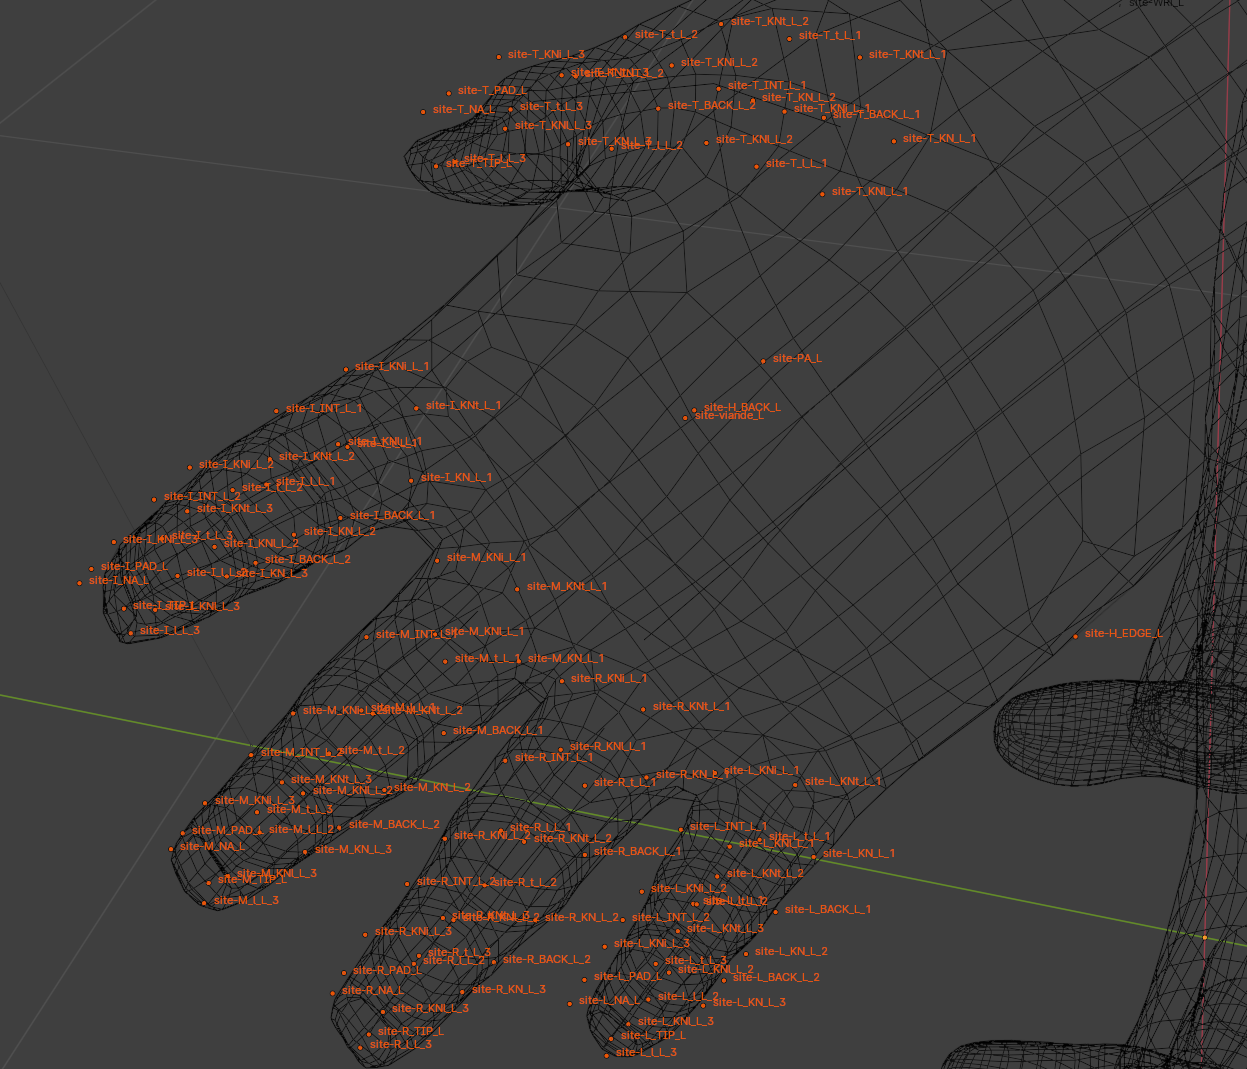
\includegraphics[width=\textwidth]{chapters/avatar_creation_pose_synthesis/images/sites_hand.png}
        \caption{Hand Sites}
        \label{fig:sites_hand}
    \end{subfigure}
    \caption{AZee sites on the BAZeel avatar: Front and Back Body Views, and Hand Sites}
    \label{fig:sites_bazeel_combined}
\end{figure}

\subsection{Creating the bone heirarchy}
\label{ch:avatar_creation_pose_synthesis:proc_rig_signing_avatars:bone_layers}

The previous system only used an armature with rotation and translation bones (explained in section~\ref{ch:background_work:sign_language_synthesis:3d_techniques:sign_language_synthesis_systems:azee_based:low_level_synthesizer_for_azee:bone_heirarchy}). We chose to work from mixamo (section~\ref{ch:background_work:sign_language_synthesis:3d_techniques:skeleton:mixamo}) based avatar skeletons and also use account for mesh deformity based on the constraints. To address this, we used bone layers to organize the bones into separate groups based on their function and purpose. Bone layers are often used in 3D animation software to organize and manage bones in a rig. By grouping bones into separate layers, animators can control which bones are visible and selectable at any given time, making it easier to work with complex rigs and animations. The new system has 3 types of bone layers: the deformation bone layer, the \gls{ik} layer, and the \gls{fk} layer.

\subsubsection{Deformation Bone Layer}
\label{ch:avatar_creation_pose_synthesis:proc_rig_signing_avatars:bone_layers:deform_bone_layer}

The deformation bone layer (figure~\ref{fig:deform_layer}) is the foundation of the avatar's rig. It includes the bones that directly influence the mesh of the character, controlling how the skin deforms in response to movement. This layer is responsible for the overall shape and posture of the avatar, ensuring that the character's movements are smooth and realistic.

In this layer, the bones are typically organized into a hierarchy, with the root bone controlling the overall position and orientation of the avatar, and child bones controlling specific parts of the body, such as the limbs, spine, and head. Weight painting is used to determine how much influence each bone has over the surrounding mesh, allowing for precise control over how the character's skin deforms.

\begin{figure}
    \centering
    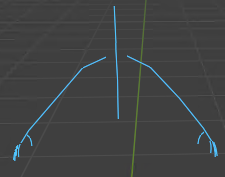
\includegraphics[width=0.5\textwidth]{chapters/avatar_creation_pose_synthesis/images/deform_layer.png}
    \caption{Deformation bone layer}
    \label{fig:deform_layer}
\end{figure}

\subsubsection{FK Layer}
\label{ch:avatar_creation_pose_synthesis:proc_rig_signing_avatars:bone_layers:fk_layer}

The \gls{fk} layer (figure~\ref{fig:fk_layer}) controls the rotation of bones in a hierarchical manner, where the rotation of a parent bone affects all its children. This layer is used for broader, more deliberate movements, such as head tilts, body leans, or full-body rotations.

\gls{fk} provides animators with a high degree of control over each individual bone in the rig, allowing for precise adjustments to the character's pose. Unlike \gls{ik}, where the position of the end effector is specified, \gls{fk} requires the animator to manually rotate each bone in the chain, starting from the root and working down to the extremities. This can be more time-consuming but offers greater flexibility in achieving complex poses.

\begin{figure}[h]
    \centering
    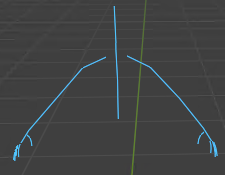
\includegraphics[width=0.3\textwidth]{chapters/avatar_creation_pose_synthesis/images/fk_layer.png}
    \caption{FK bone layer}
    \label{fig:fk_layer}
\end{figure}

\subsubsection{IK Layer}
\label{ch:avatar_creation_pose_synthesis:proc_rig_signing_avatars:bone_layers:ik_layer}

The \gls{ik} layer (figure~\ref{fig:ik_layer}) is responsible for positioning the avatar's fingers, limbs and spine by solving for the joint angles required to achieve a desired end-effector position.

A separate \gls{ik} layer ensures that the \gls{fk} configuration is not lost during constraint evaluation. If the posture is in \gls{ik} mode i.e. is solving for a placement, the deform layers copy the orientations resolved by the \gls{ik} layer.

\begin{figure}[h]
    \centering
    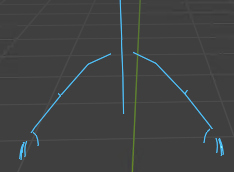
\includegraphics[width=0.4\textwidth]{chapters/avatar_creation_pose_synthesis/images/ik_layer.png}
    \caption{IK bone layer}
    \label{fig:ik_layer}
\end{figure}

\subsection{Constraint Based Posture Optimization}
\label{ch:avatar_creation_pose_synthesis:proc_rig_signing_avatars:cb_posegen}

The previous low level synthesizer for AZee used a constraint based optimization algorithm (explained in section~\ref{ch:background_work:sign_language_synthesis:3d_techniques:sign_language_synthesis_systems:azee_based:low_level_synthesizer_for_azee:pose_generation} of chapter~\ref{ch:background_work}) to generate the armature pose for a frame. This algorithm collects all posture constraints given by the AZee Animated Score for every frame and solves for the posture by optimizing these constraints using distance functions. 

However, their approach handles only placements and orientations and uses a flattened animated AZee Score. We improved on this using the algorithm~\ref{alg:trimmed_optimization} by generating from the multi-track synced score itself (explained in section~\ref{ch:background_work:sign_language_descriptions:azee:representation}). We also added support for other constraints such as \emph{morph}, \emph{lookat} and \emph{trill}.

\begin{algorithm}
    \caption{Constraint-Based Optimization for Posture Synthesis}
    \label{alg:trimmed_optimization}
    \begin{algorithmic}[1]
        \Require $\mathit{posture\_constraint\_DAG}$, $\mathit{armature\_object}$, $\mathit{frames}$
        \Ensure Armature object posed per constraints
        
        \State \textbf{Initialize:} $i \gets 0$, $max\_iterations \gets \mathit{scene.max\_iterations}$
        \State $\mathit{sorted\_constraints} \gets \mathit{posture\_constraint\_DAG.sort()}$, $\mathit{frames\_to\_keyframe} \gets \textsc{DetermineFrames}(\mathit{frames})$
        
        \While{$i < max\_iterations$}
            \ForAll {$f \in \mathit{frames\_to\_keyframe}$}
                \State $\mathit{loss} \gets 0$
                \ForAll {$constraint \in \mathit{sorted\_constraints}$}
                    \State \textsc{ApplyConstraint}($constraint$, $f$)
                    \State $\mathit{loss} \gets loss + \mathit{constraint.get\_loss(f)}$
                \EndFor
                \If {$loss < \mathit{scene.threshold}$}
                    \State \textbf{Break}
                \EndIf
                \State \textsc{InsertKeyframe}($f$)
            \EndFor
            \State $i \gets i + 1$
        \EndWhile
        
        \Procedure{ApplyConstraint}{$constraint, f$}
            \If {$constraint$ \textbf{is} PlacementConstraint}
                \State \textsc{PlaceSite}($constraint.site$, \textsc{EvaluatePlacementTarget}($constraint$, $f$))
            \ElsIf {$constraint$ \textbf{is} OrientationConstraint}
                \State \textsc{RotateBone}($constraint.bone$, \textsc{EvaluateOrientation}($constraint$, $f$))
            \Else
                \State \textsc{HandleError}()
            \EndIf
        \EndProcedure
        
        \Procedure{InsertKeyframe}{$f$}
            \ForAll {$fcurve \in \mathit{armature\_object.animation\_data.fcurves}$}
                \State \textsc{KeyframeInsert}($fcurve$, $f$)
            \EndFor
        \EndProcedure
    \end{algorithmic}
\end{algorithm}

\subsection{Joint Limits}
\label{ch:avatar_creation_pose_synthesis:proc_rig_signing_avatars:joint_limits}

To prevent the avatar from entering physically impossible poses, we assigned joint limit constraints to the skeleton. These joint limits ensure that the avatar adheres to natural anatomical boundaries, avoiding extreme or unnatural movements like hyperextension or hyperflexion beyond what is realistically possible for human joints.

Joint limits help guide the skeleton during animation, particularly when the system uses inverse kinematics or procedural rigging, by ensuring that no joint moves beyond its allowed range. For instance, finger joints such as the \gls{mcp}, \gls{pip}, and \gls{dip} joints have defined ranges of motion that prevent unrealistic bending or rotation.

An example of the joint limits applied to the \gls{mcp}, \gls{pip}, and \gls{dip} joints in the fingers is visualized in Figure~\ref{fig:joint_limits_finger}. The plot demonstrates the flexion and extension limits for each of these joints.

\begin{figure}[h!]
    \centering
    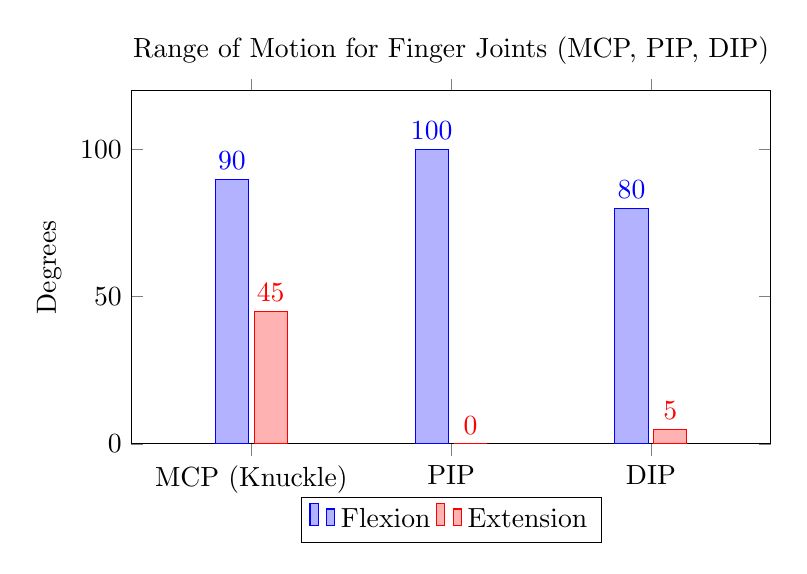
\begin{tikzpicture}
    \begin{axis}[
        width=0.8\textwidth,
        height=0.5\textwidth,
        symbolic x coords={MCP (Knuckle), PIP, DIP},
        xtick=data,
        ymin=0, ymax=120,
        bar width=12pt,
        ybar,
        xlabel={Finger Joint},
        ylabel={Degrees},
        nodes near coords,
        enlarge x limits=0.3,
        legend style={at={(0.5,-0.15)},anchor=north,legend columns=-1},
        title={Range of Motion for Finger Joints (MCP, PIP, DIP)}
    ]
        \addplot coordinates {(MCP (Knuckle),90) (PIP,100) (DIP,80)};
        \addplot coordinates {(MCP (Knuckle),45) (PIP,0) (DIP,5)};
        \legend{Flexion, Extension}
    \end{axis}
    \end{tikzpicture}
    \caption{Range of motion for finger joints showing the flexion and extension limits for MCP, PIP, and DIP joints.}
    \label{fig:joint_limits_finger}
\end{figure}

Joint limit constraints ensure that each joint, including those in the fingers, remains within the specified anatomical range of motion, as visualized in Figure~\ref{fig:joint_limits_finger}. This prevents the avatar from adopting poses that would be physically impossible or cause damage in real-life scenarios.

\subsection{Animating Morphs Constraints}
\label{ch:avatar_creation_pose_synthesis:proc_rig_signing_avatars:morph_constraints}

The word "morph" comes from the Greek word \textit{morphē}, which means "form" or "shape." In modern usage, "morph" is often used as a shorthand for "morphing." In the field of computer graphics and animation, morphs are predefined shape keys that modify the mesh of the avatar independently of the skeletal structure, allowing for a fine control of the avatar's appearance that cannot be easily achieved through bone manipulation alone. This includes subtle facial expressions, muscle bulges, and other nuanced gestures that are critical for conveying meaning in \gls{sl}.

AZee didn't have any morph specification to control the avatar. During this work, we populated them with skeletal and facial morphs. These morphs are changes in the configuration of the avatar, which can be specified by the linguist in a range from 0 to 1. For instance, closing of hands(a change in skeleton configuration) or raising the eyebrows(a change in the 3D mesh). The syntax of a morph constraint is as follows:

\[
\texttt{morph } \text{\emph{'morph\_id'}} \ \texttt{weight[0, 1]}
\]

\subsubsection{Skeletal Morphs}
\label{ch:avatar_creation_pose_synthesis:proc_rig_signing_avatars:morph_constraints:skel_morphs}

Skeletal morphs are a specific type of morphs that directly manipulate the skeletal structure of an avatar to produce a desired pose or motion. Unlike traditional bone-based manipulations that rely solely on inverse or \gls{fk}, skeletal morphs allow for more nuanced and localized control over specific joints or groups of joints. This is particularly useful for complex hand gestures or other detailed movements that are difficult to achieve with bone rotations alone.

In AZee, skeletal morphs are treated as constraints that define a forward kinematic change in the avatar's skeletal configuration. These morphs can influence various aspects of the skeleton, such as:

\begin{itemize}
    \item \textbf{Flexion and Extension:} This refers to the bending (flexion) or straightening (extension) of a joint (figure~\ref{fig:hyper-extension_flexion}), such as the fingers or wrists. Flexion reduces the angle between bones, while extension increases it.
    \item \textbf{Adduction and Abduction:} Adduction involves moving a limb closer to the body's midline (figure~\ref{fig:adduction_abduction}), whereas abduction moves it away. These movements are crucial for natural arm and hand gestures.
    \item \textbf{Hyperextension:} This is an extension of a joint beyond its normal range of motion (figure~\ref{fig:hyper-extension_flexion}), often used for expressive gestures that require exaggerated poses.
\end{itemize}

\begin{figure}
    \centering
    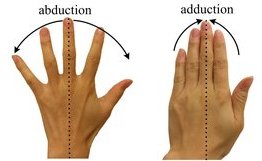
\includegraphics[width=0.5\textwidth]{chapters/avatar_creation_pose_synthesis/images/adduction_abduction.jpg}
    \caption{Adduction and Abduction of the palm}
    \label{fig:adduction_abduction}
\end{figure}

\begin{figure}
    \centering
    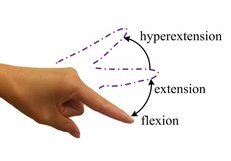
\includegraphics[width=0.5\textwidth]{chapters/avatar_creation_pose_synthesis/images/hyper-extension_flexion.jpg}
    \caption{Flextion and Hyperextension of the index finger}
    \label{fig:hyper-extension_flexion}
\end{figure}

Figure~\ref{fig:skeletal_morphs} shows a table of skeletal morphs and their corresponding effects on the avatar's skeleton.

\begin{figure}
    \centering
    \begin{tabular}{|c|c|c|c|}
        \hline
        \textbf{Left Morphs (L)} & \textbf{Effect} & \textbf{Right Morphs (R)} & \textbf{Effect} \\ 
        \hline
        % Finger Morphs
        \texttt{index\_bend\_L} & 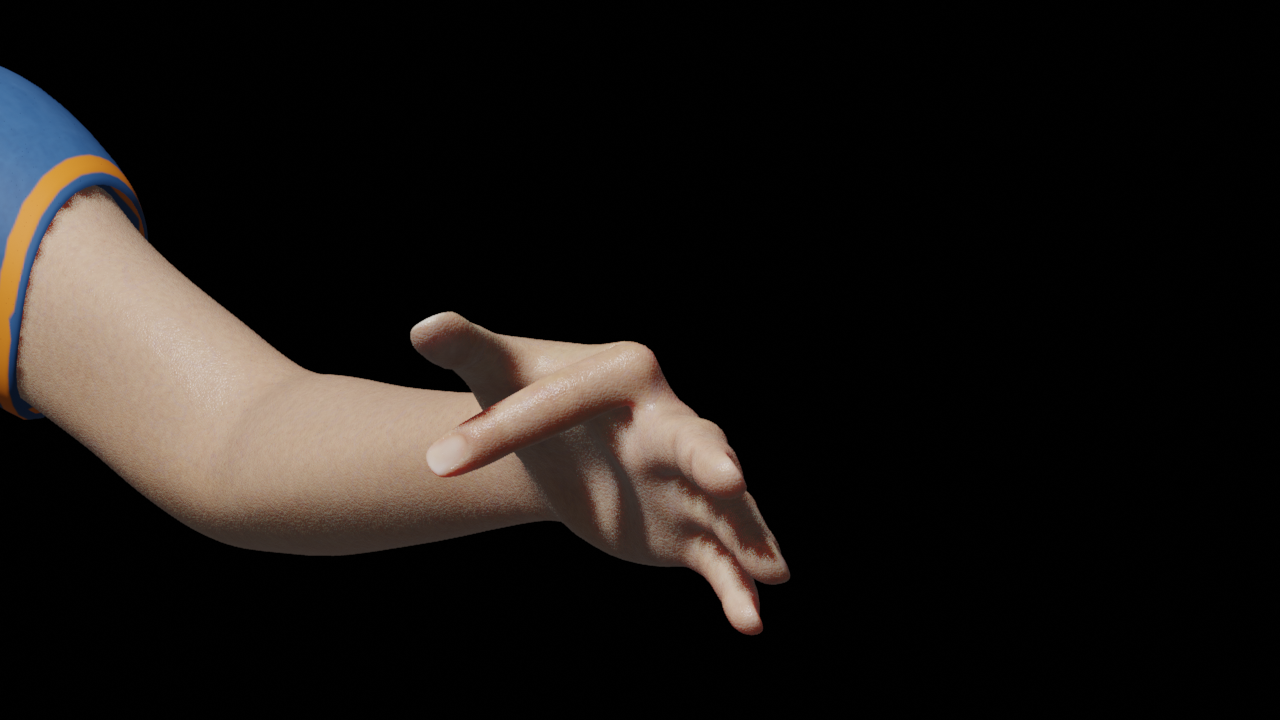
\includegraphics[width=0.1\textwidth]{chapters/avatar_creation_pose_synthesis/images/morph_renders/index_bend_L_morph.png} & 
        \texttt{index\_bend\_R} & 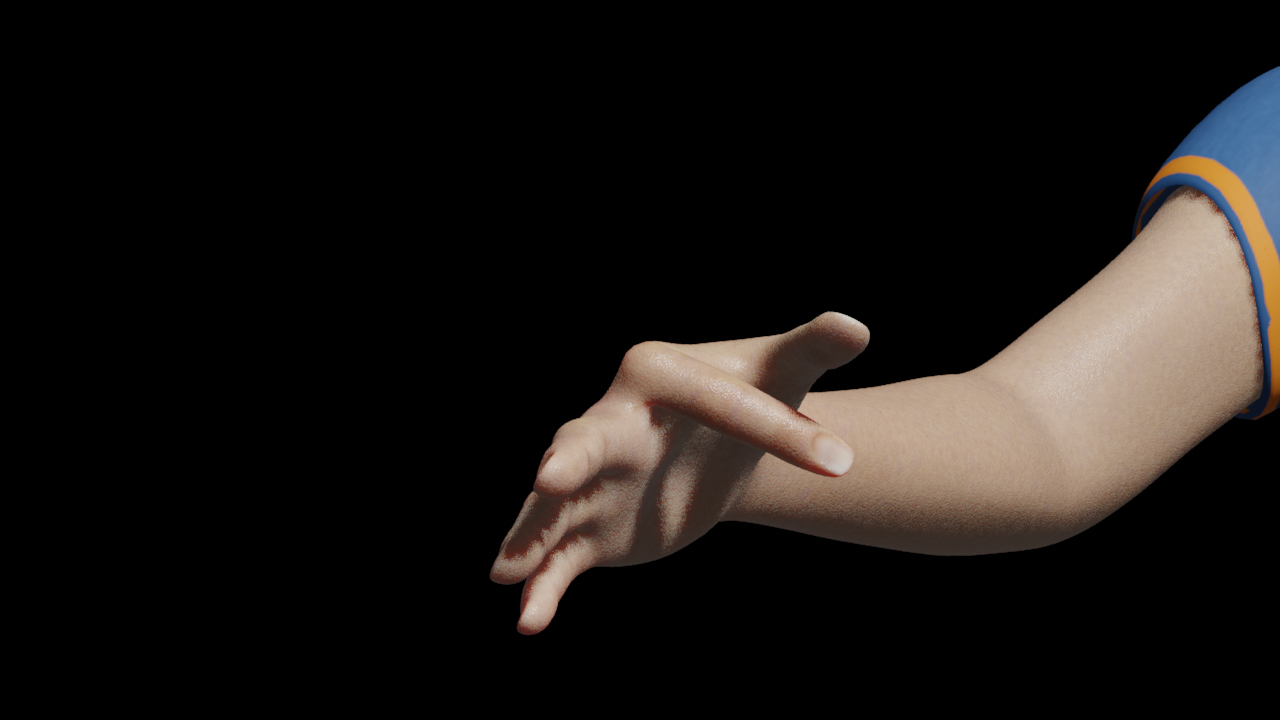
\includegraphics[width=0.1\textwidth]{chapters/avatar_creation_pose_synthesis/images/morph_renders/index_bend_R_morph.png} \\

        \texttt{middle\_bend\_L} & 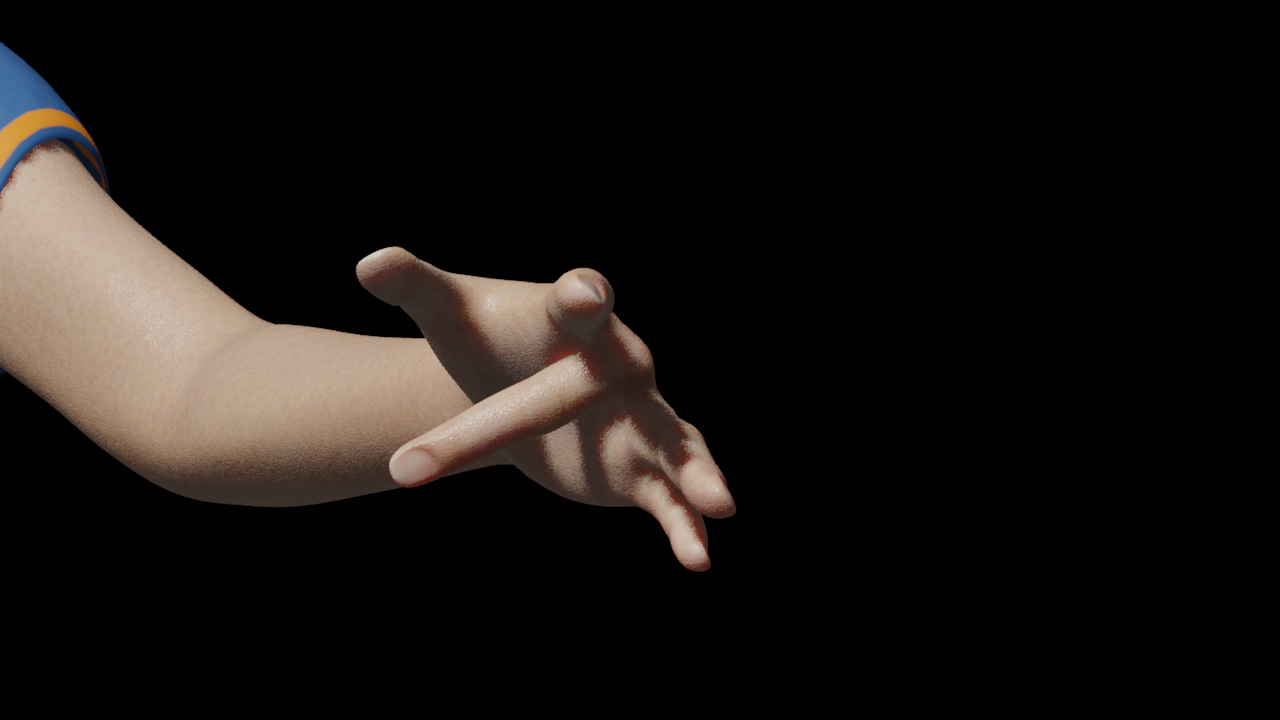
\includegraphics[width=0.1\textwidth]{chapters/avatar_creation_pose_synthesis/images/morph_renders/middle_bend_L_morph.png} &
        \texttt{middle\_bend\_R} & 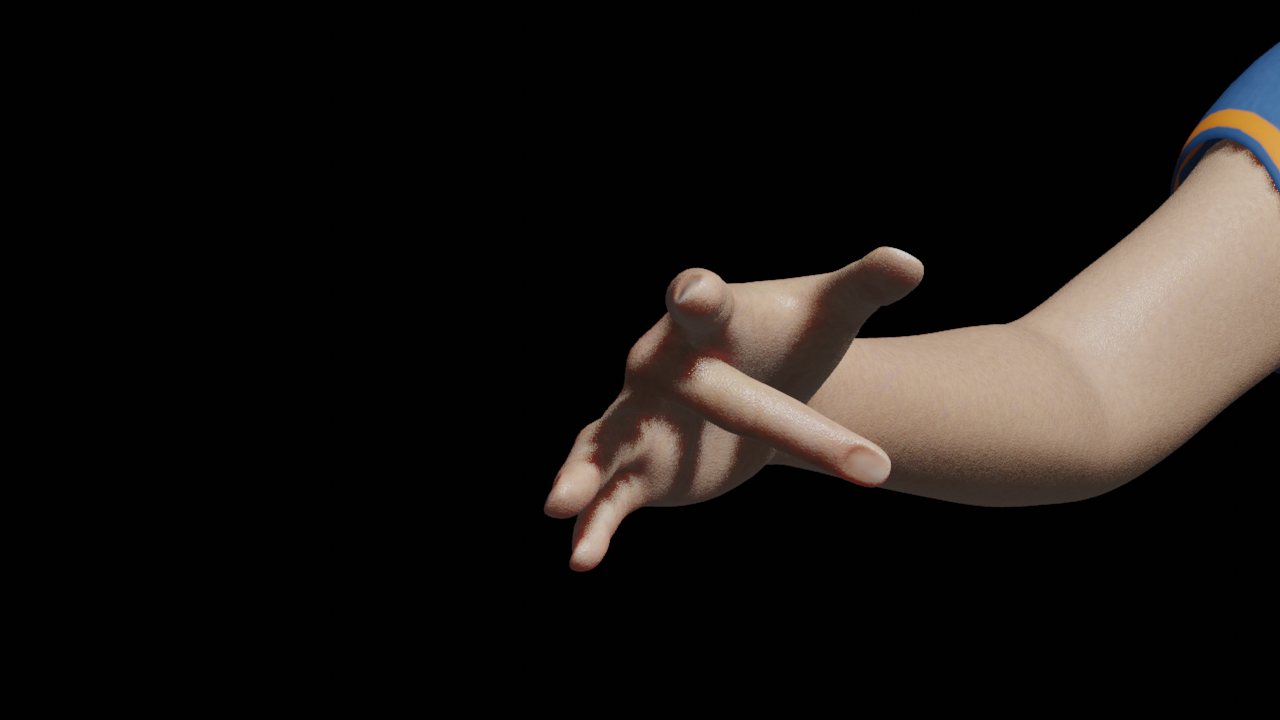
\includegraphics[width=0.1\textwidth]{chapters/avatar_creation_pose_synthesis/images/morph_renders/middle_bend_R_morph.png} \\

        \texttt{ring\_bend\_L} & 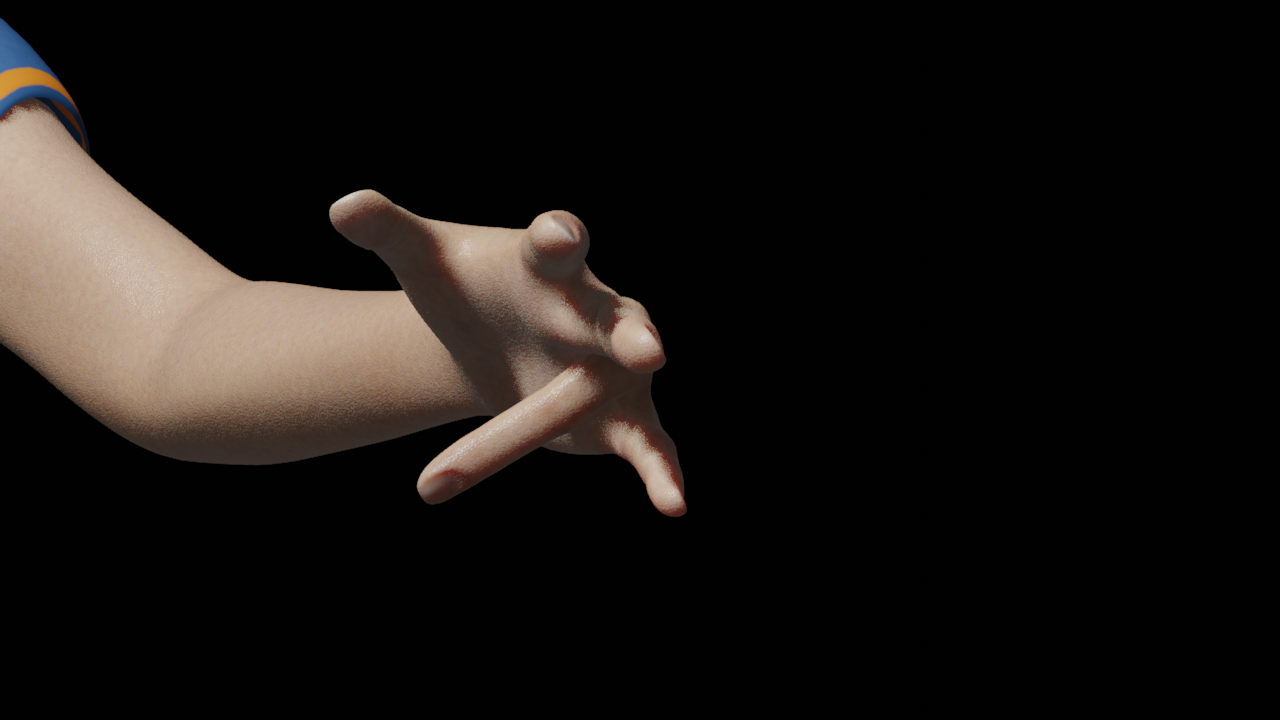
\includegraphics[width=0.1\textwidth]{chapters/avatar_creation_pose_synthesis/images/morph_renders/ring_bend_L_morph.png} &
        \texttt{ring\_bend\_R} & 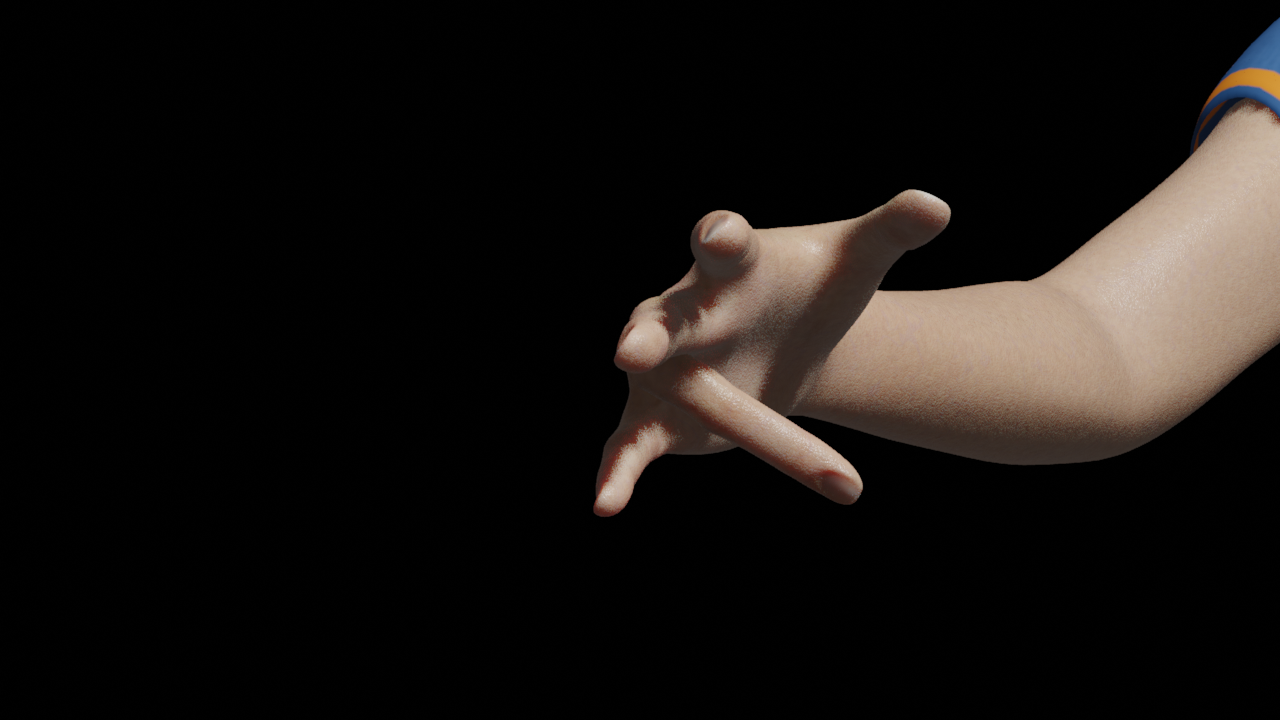
\includegraphics[width=0.1\textwidth]{chapters/avatar_creation_pose_synthesis/images/morph_renders/ring_bend_R_morph.png} \\

        \texttt{little\_bend\_L} & 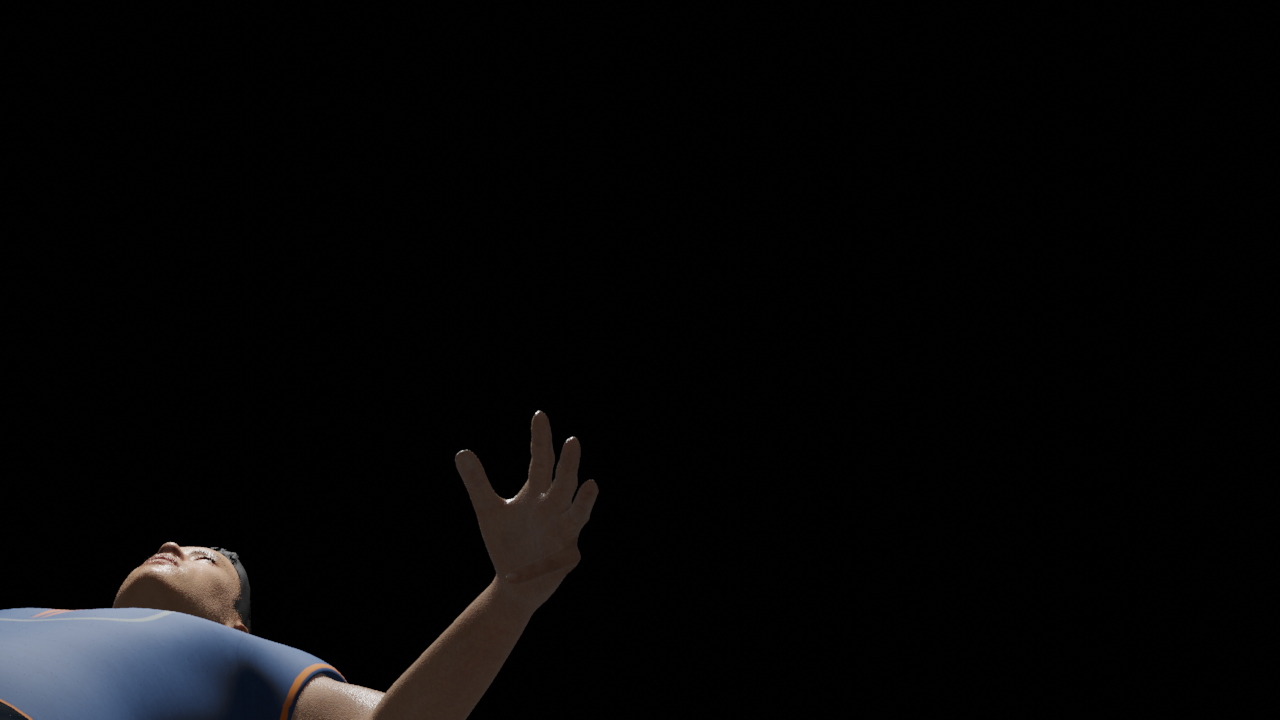
\includegraphics[width=0.1\textwidth]{chapters/avatar_creation_pose_synthesis/images/morph_renders/little_bend_L_morph.png} & 
        \texttt{little\_bend\_R} & 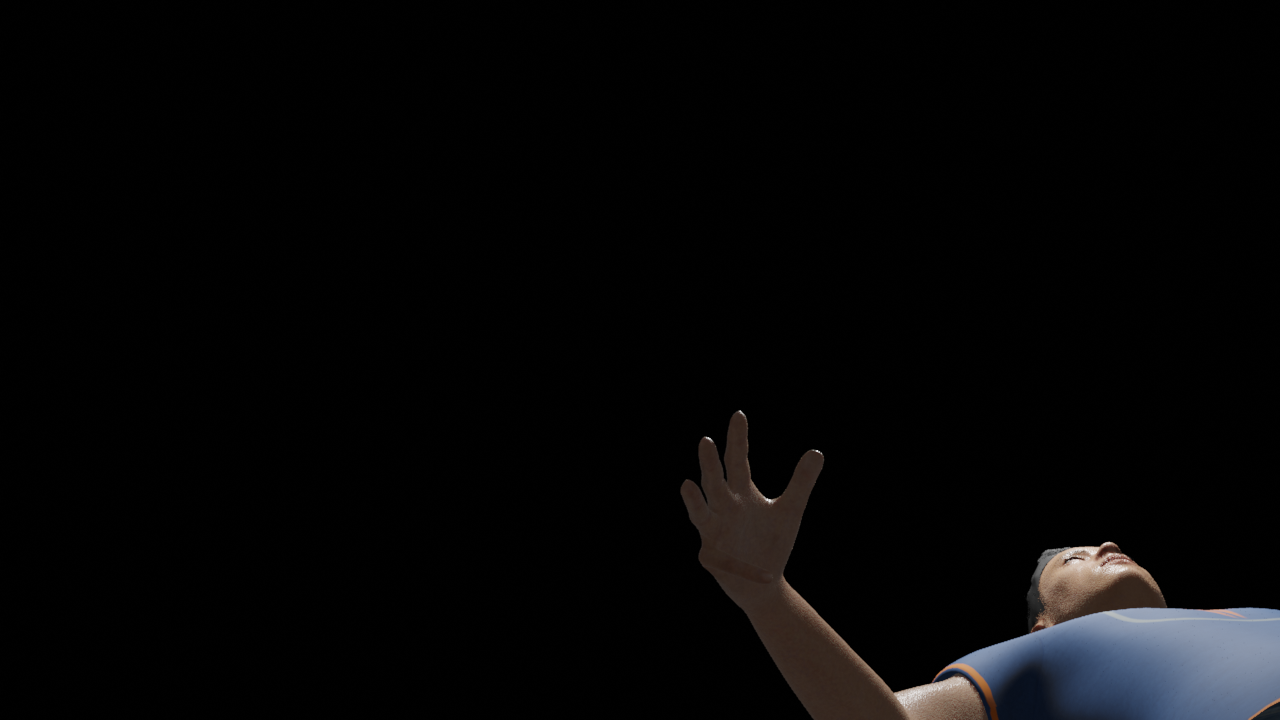
\includegraphics[width=0.1\textwidth]{chapters/avatar_creation_pose_synthesis/images/morph_renders/little_bend_R_morph.png} \\

        \texttt{index\_hook\_L} & 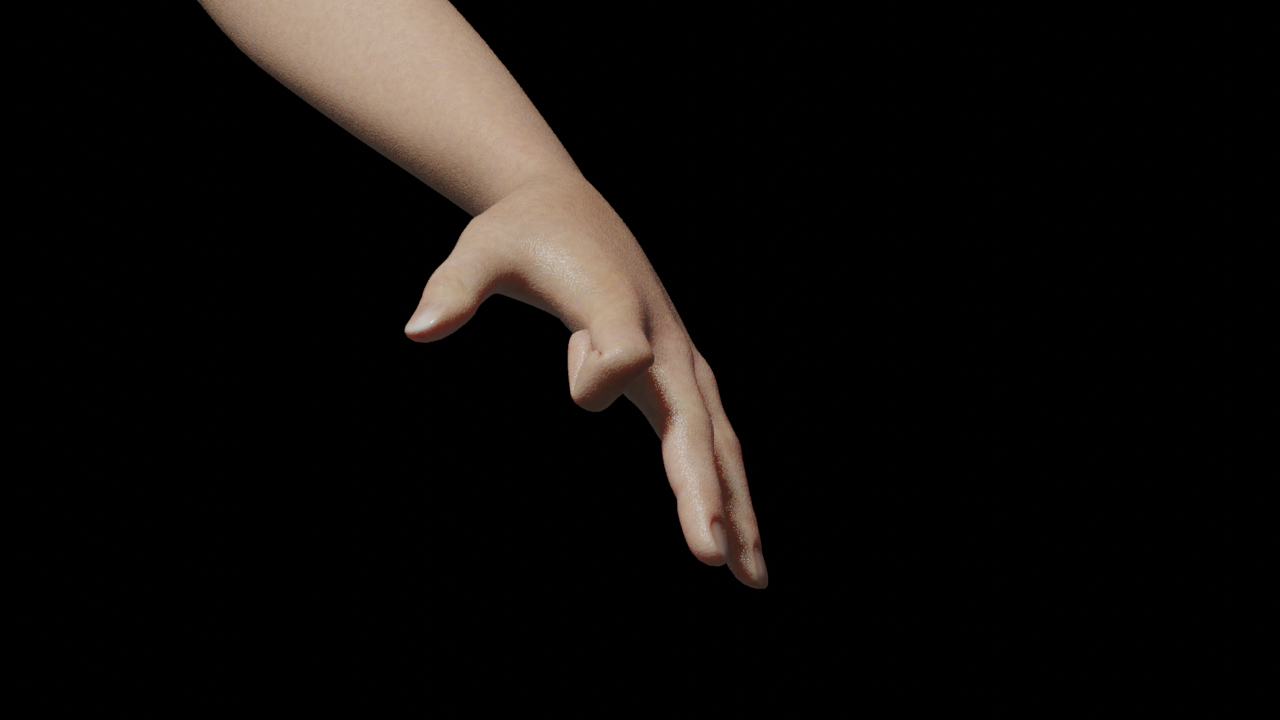
\includegraphics[width=0.1\textwidth]{chapters/avatar_creation_pose_synthesis/images/morph_renders/index_hook_L_morph.png} &
        \texttt{index\_hook\_R} & 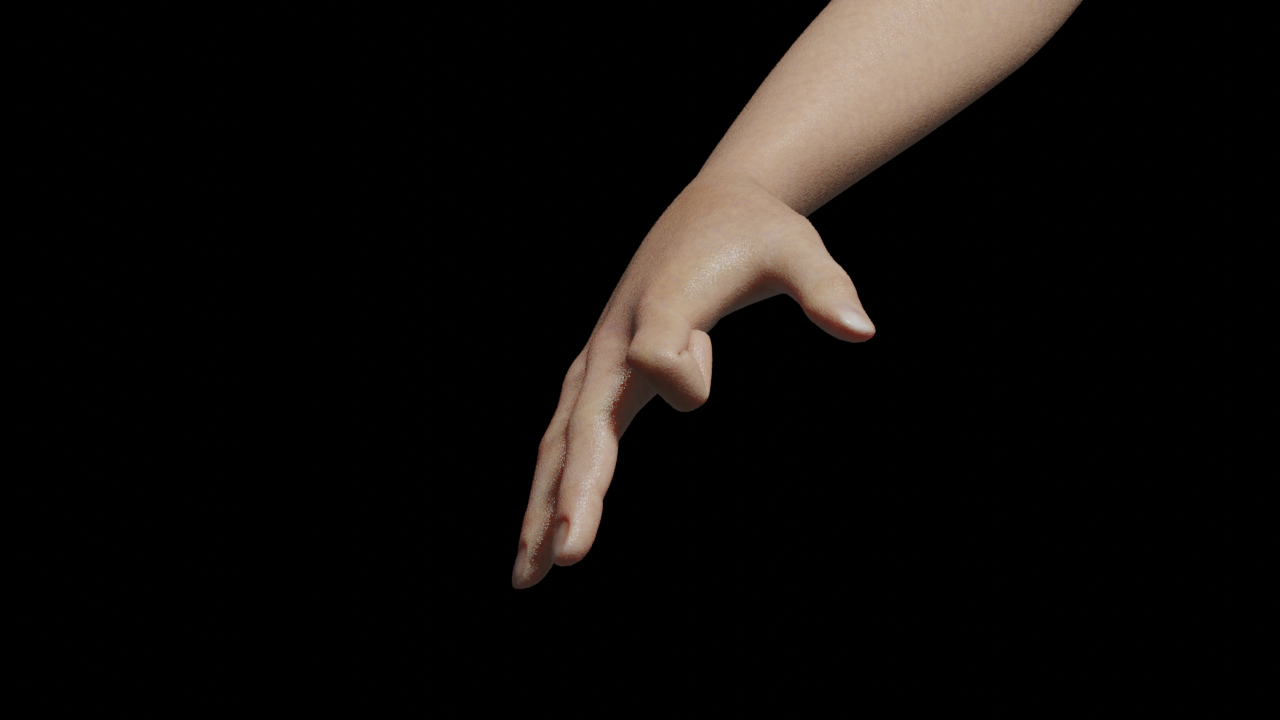
\includegraphics[width=0.1\textwidth]{chapters/avatar_creation_pose_synthesis/images/morph_renders/index_hook_R_morph.png} \\

        \texttt{middle\_hook\_L} & 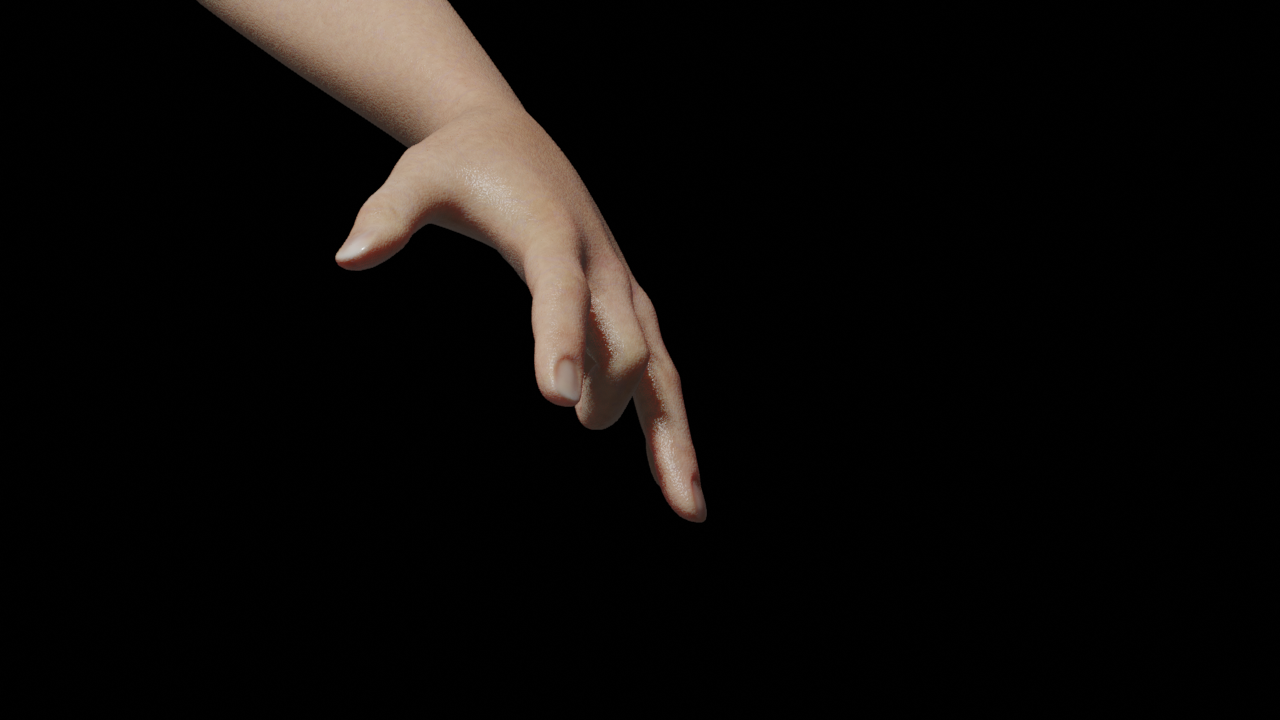
\includegraphics[width=0.1\textwidth]{chapters/avatar_creation_pose_synthesis/images/morph_renders/middle_hook_L_morph.png} & 
        \texttt{middle\_hook\_R} & 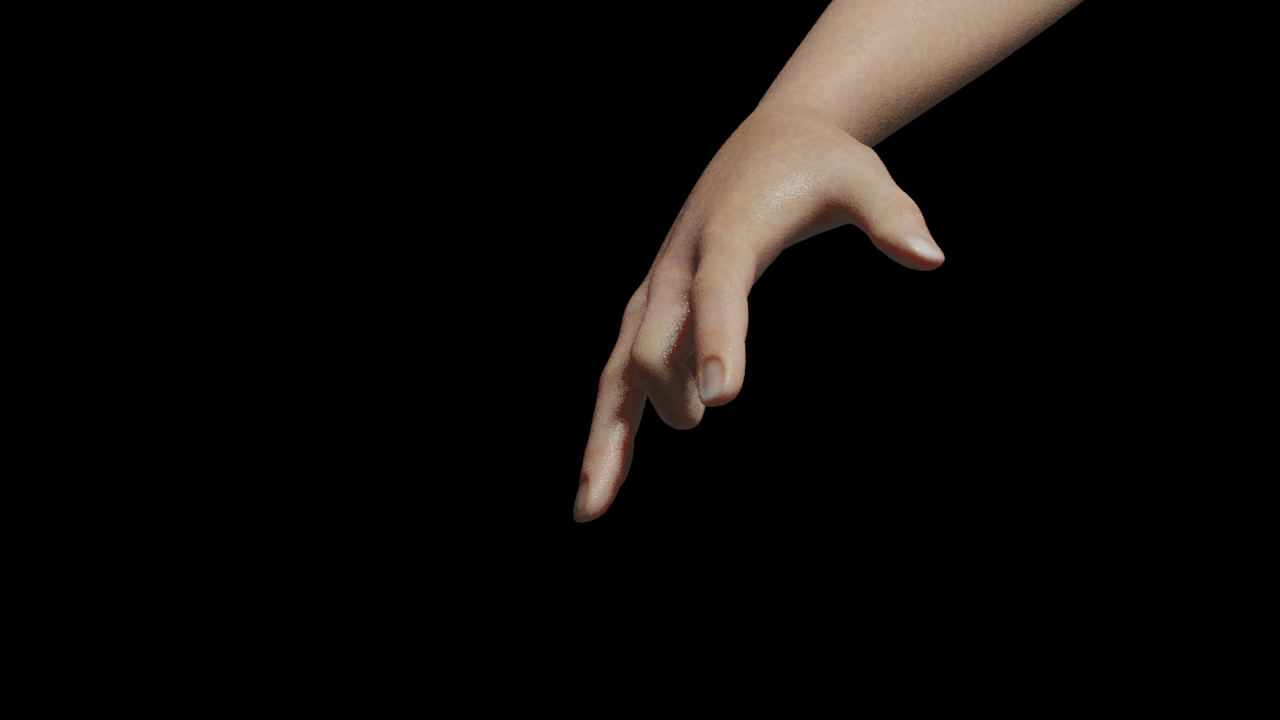
\includegraphics[width=0.1\textwidth]{chapters/avatar_creation_pose_synthesis/images/morph_renders/middle_hook_R_morph.png} \\

        \texttt{ring\_hook\_L} & 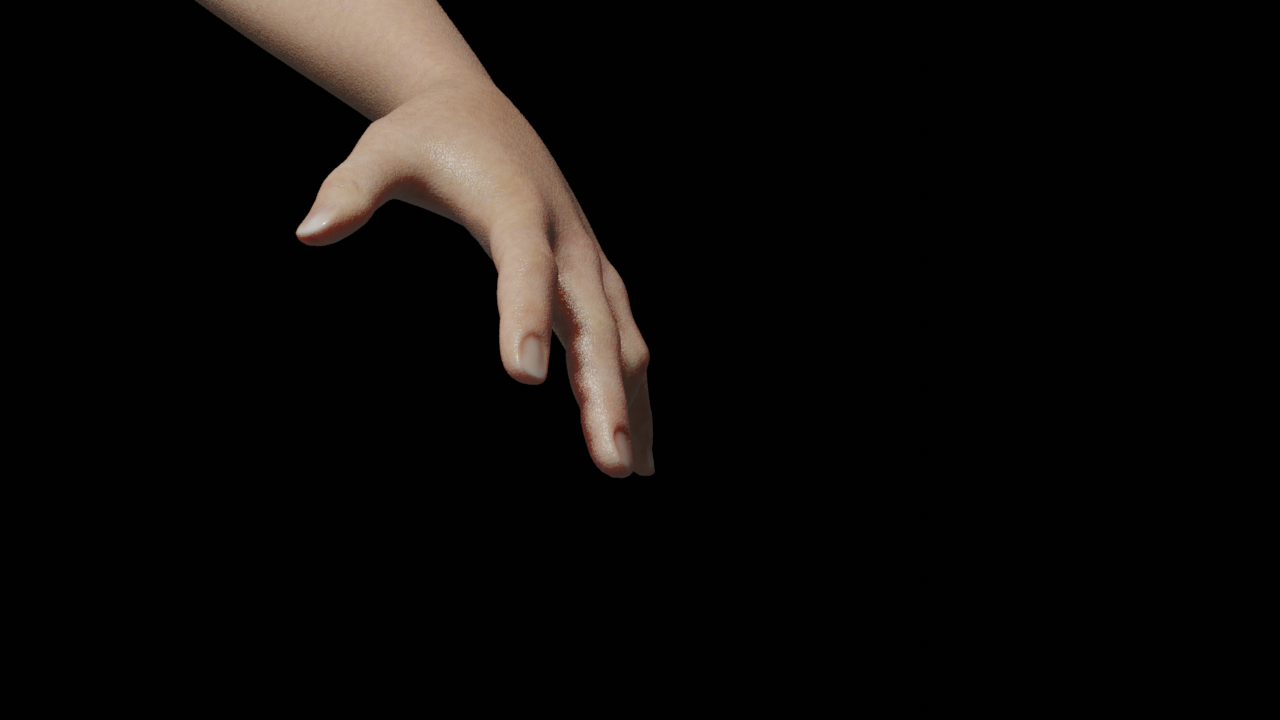
\includegraphics[width=0.1\textwidth]{chapters/avatar_creation_pose_synthesis/images/morph_renders/ring_hook_L_morph.png} &
        \texttt{ring\_hook\_R} & 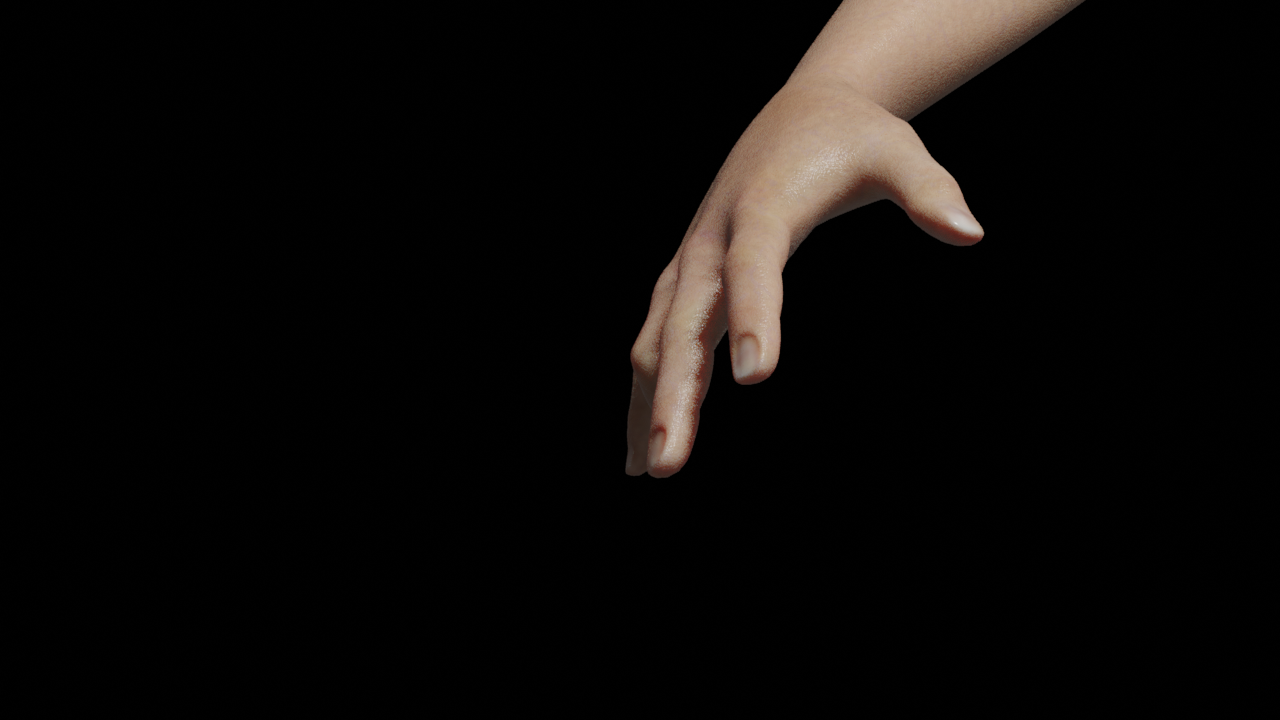
\includegraphics[width=0.1\textwidth]{chapters/avatar_creation_pose_synthesis/images/morph_renders/ring_hook_R_morph.png} \\

        \texttt{little\_hook\_L} & 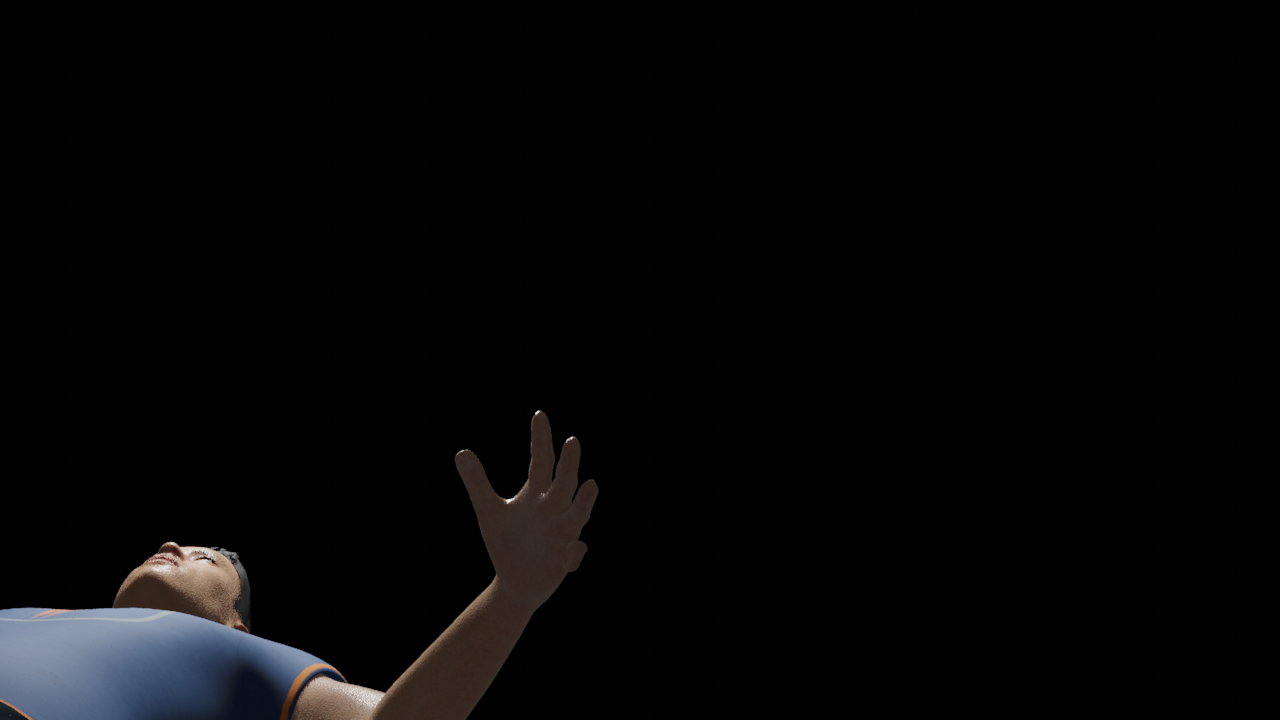
\includegraphics[width=0.1\textwidth]{chapters/avatar_creation_pose_synthesis/images/morph_renders/little_hook_L_morph.png} &
        \texttt{little\_hook\_R} & 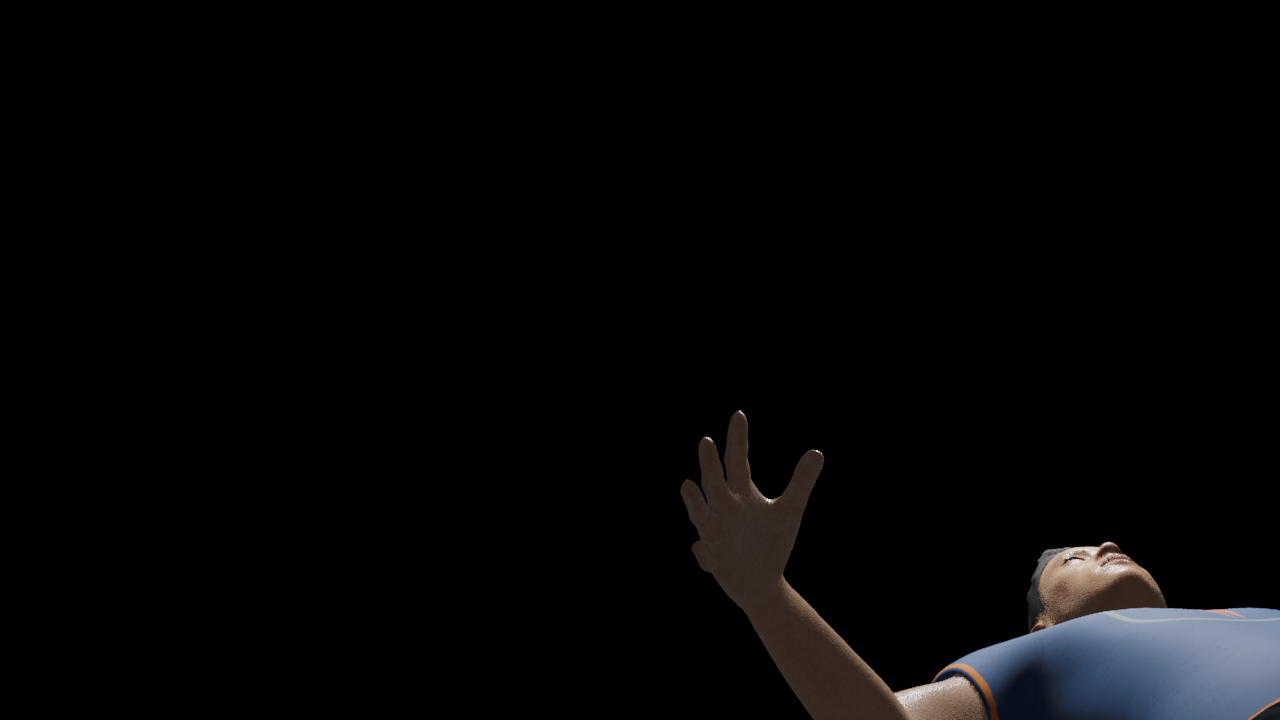
\includegraphics[width=0.1\textwidth]{chapters/avatar_creation_pose_synthesis/images/morph_renders/little_hook_R_morph.png} \\

        \texttt{thumb\_bend\_L} & 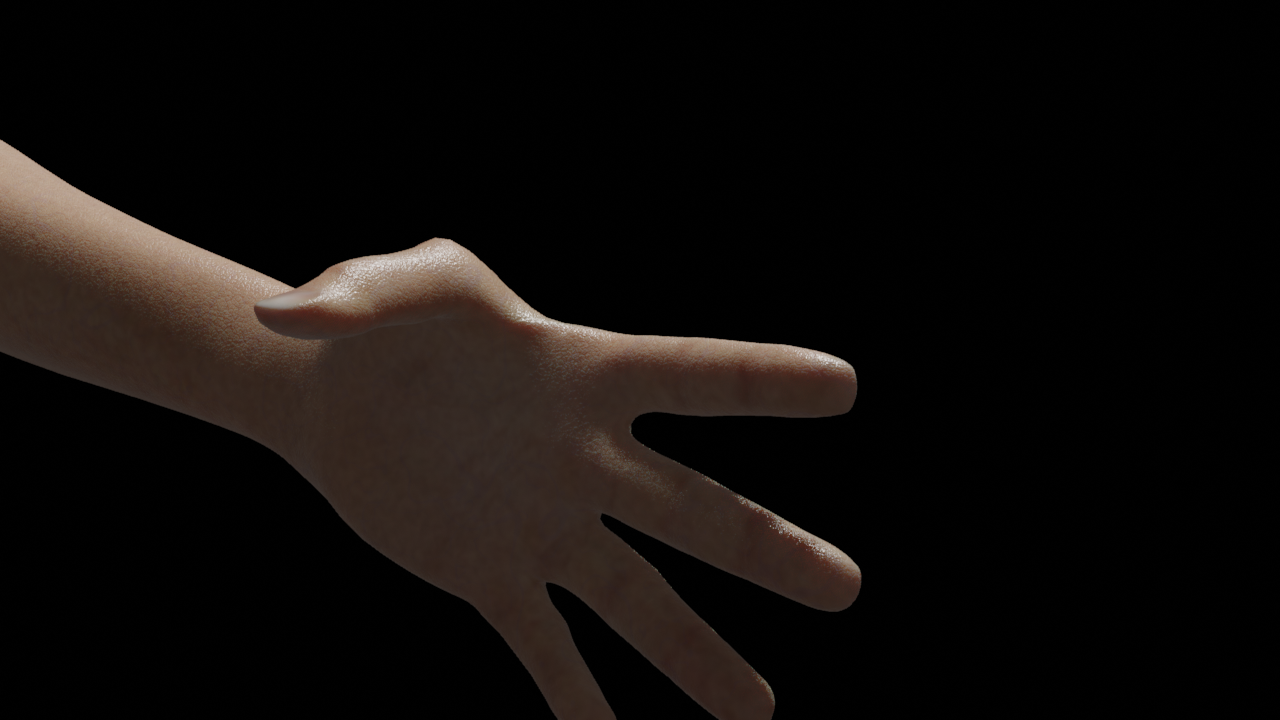
\includegraphics[width=0.1\textwidth]{chapters/avatar_creation_pose_synthesis/images/morph_renders/thumb_bend_L.png} &
        \texttt{thumb\_bend\_R} & 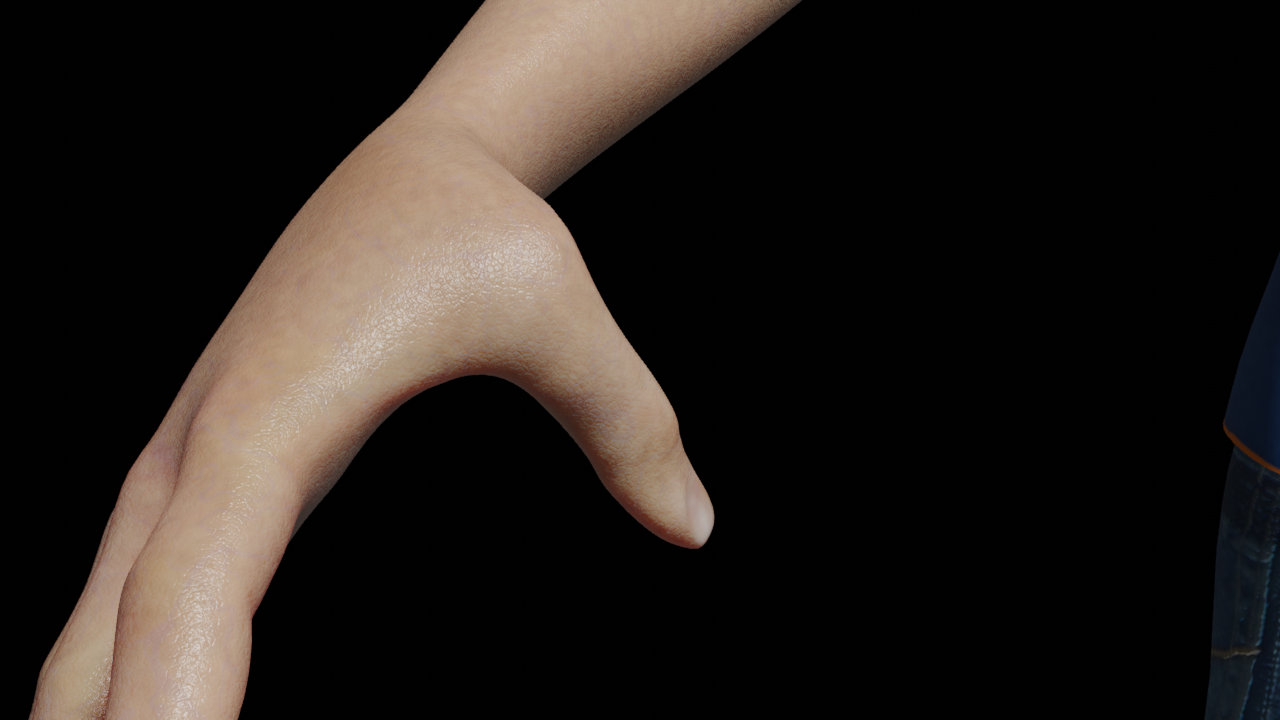
\includegraphics[width=0.1\textwidth]{chapters/avatar_creation_pose_synthesis/images/morph_renders/thumb_bend_R.png} \\

        \texttt{thumb\_hook\_L} & 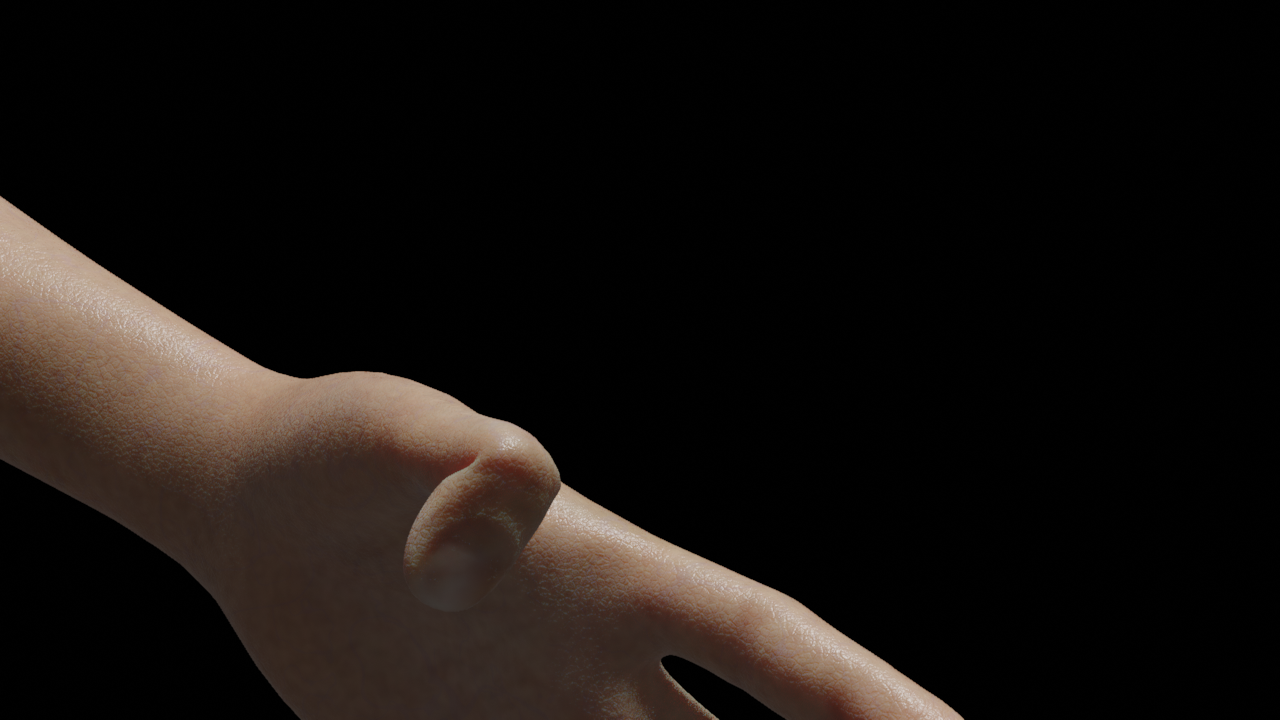
\includegraphics[width=0.1\textwidth]{chapters/avatar_creation_pose_synthesis/images/morph_renders/thumb_hook_L.png} &
        \texttt{thumb\_hook\_R} & 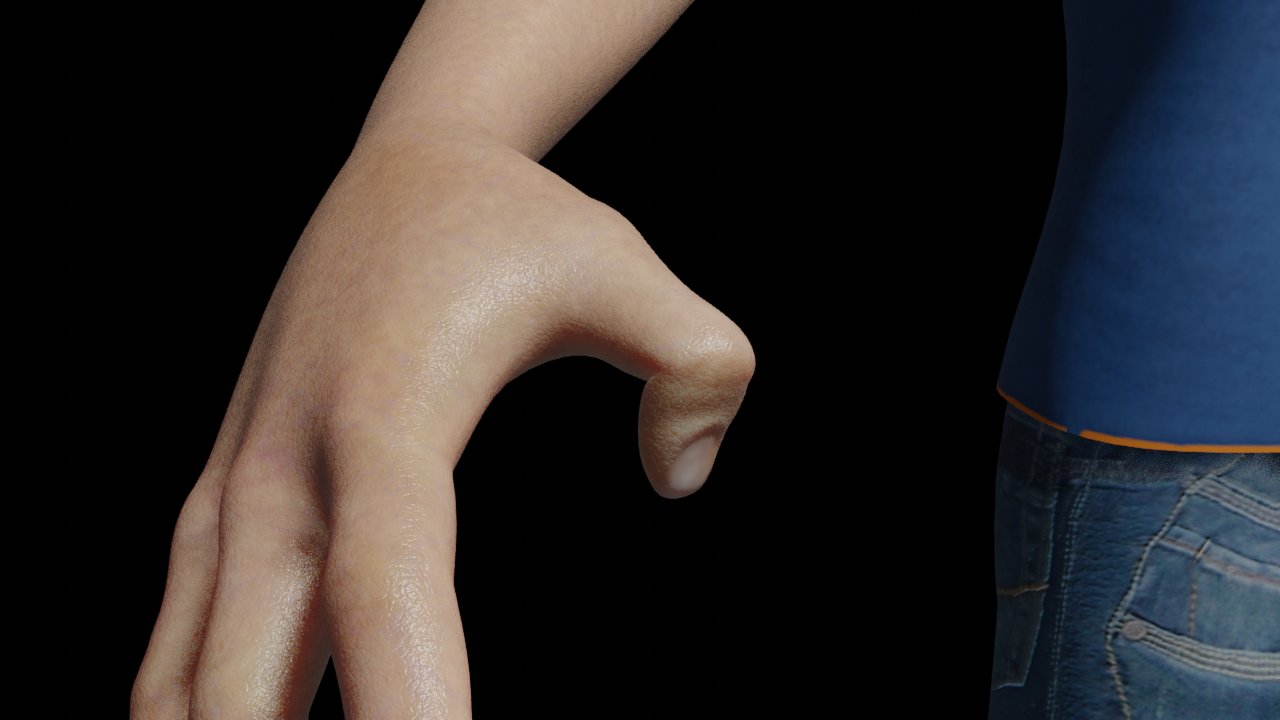
\includegraphics[width=0.1\textwidth]{chapters/avatar_creation_pose_synthesis/images/morph_renders/thumb_hook_R.png} \\

        \texttt{thumb\_opposed\_L} & 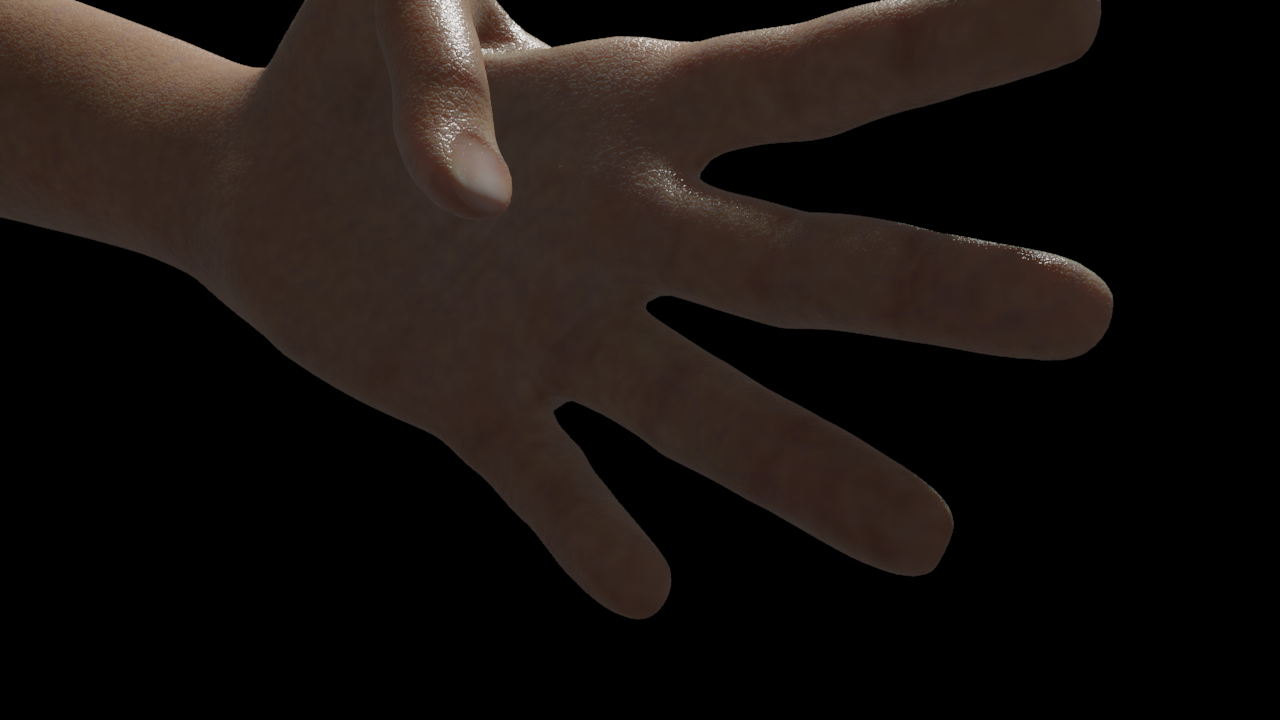
\includegraphics[width=0.1\textwidth]{chapters/avatar_creation_pose_synthesis/images/morph_renders/thumb_opposed_L.png} &
        \texttt{thumb\_opposed\_R} & 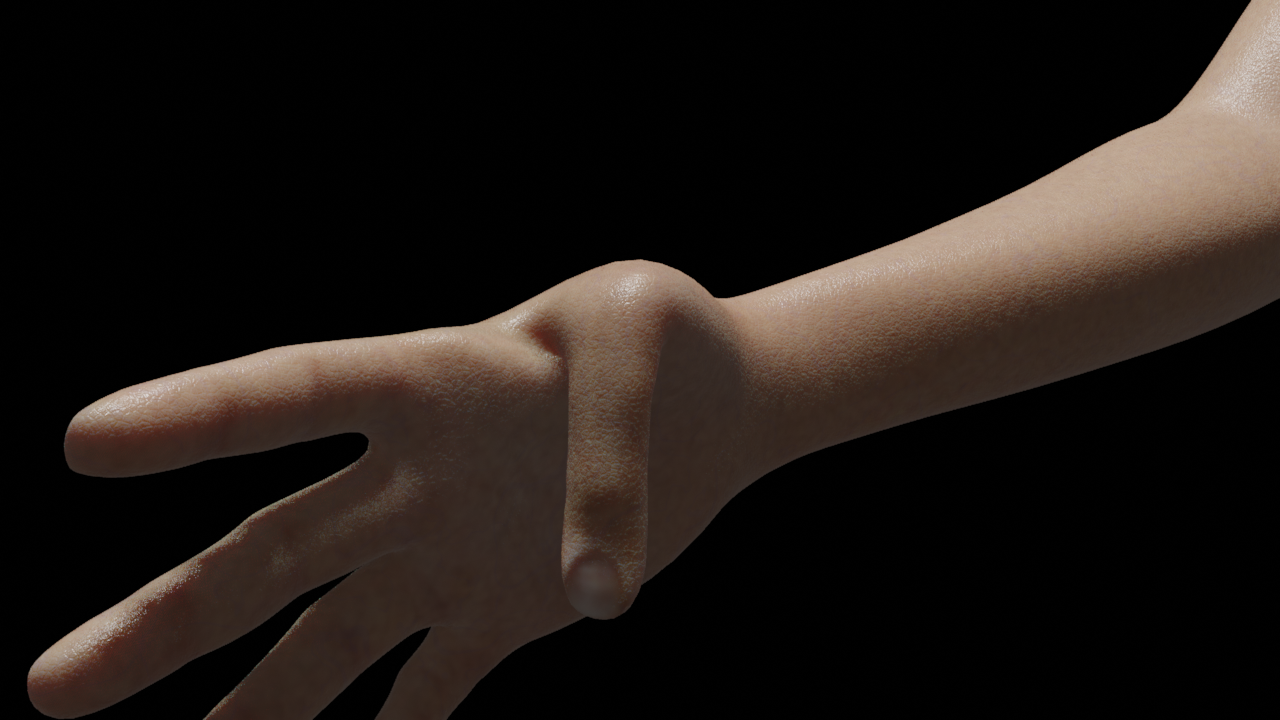
\includegraphics[width=0.1\textwidth]{chapters/avatar_creation_pose_synthesis/images/morph_renders/thumb_opposed_R.png} \\

        \texttt{thumb\_spread\_L} & 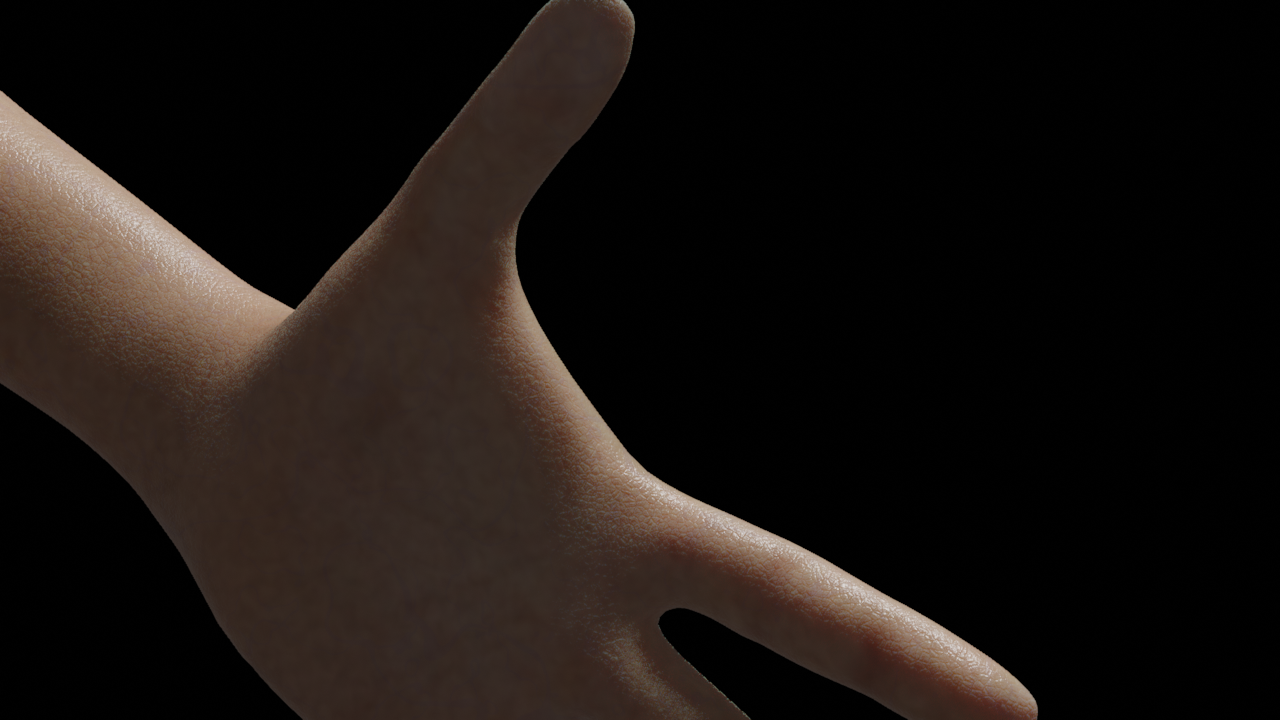
\includegraphics[width=0.1\textwidth]{chapters/avatar_creation_pose_synthesis/images/morph_renders/thumb_spread_L.png} &
        \texttt{thumb\_spread\_R} & 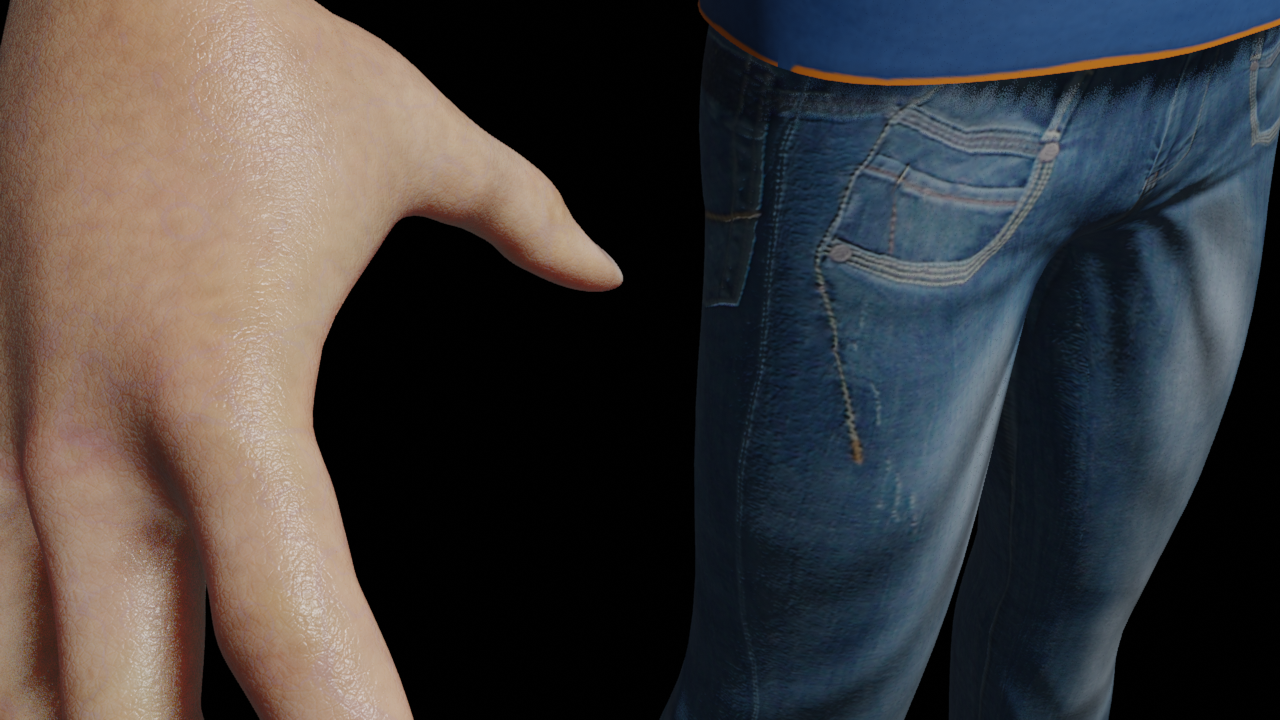
\includegraphics[width=0.1\textwidth]{chapters/avatar_creation_pose_synthesis/images/morph_renders/thumb_spread_R.png} \\

        \texttt{fingers\_spread\_L} & 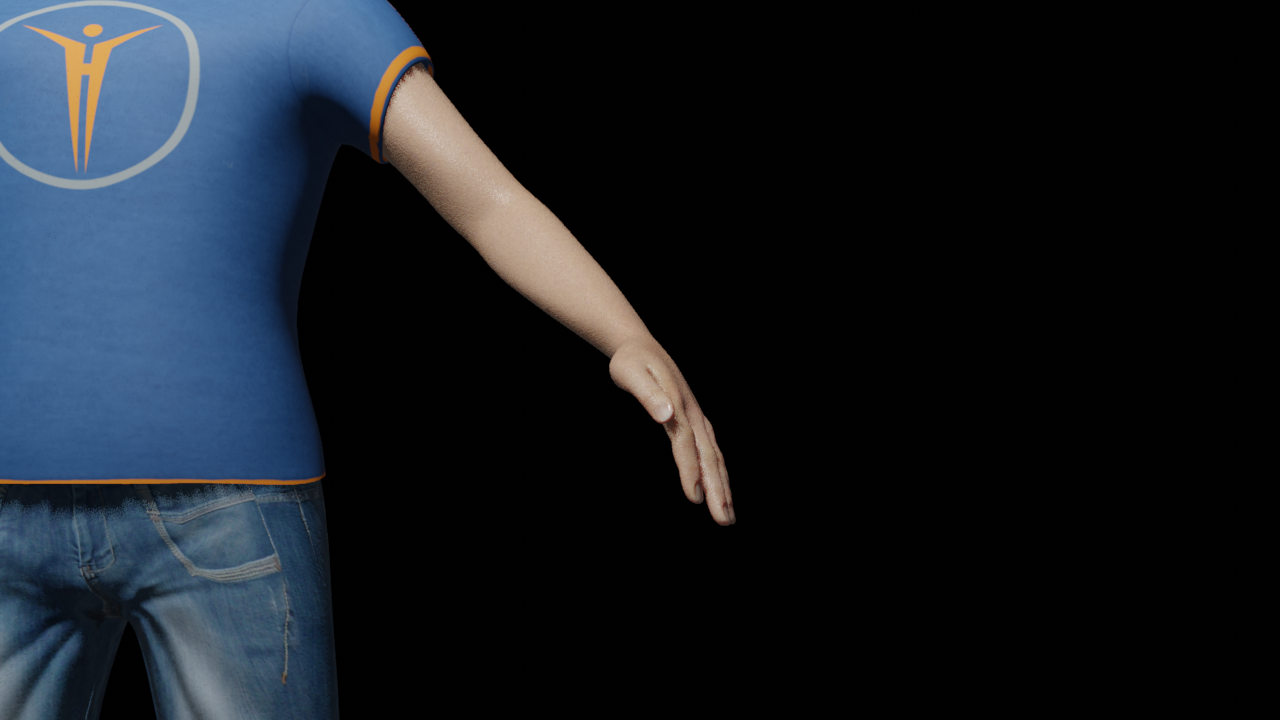
\includegraphics[width=0.1\textwidth]{chapters/avatar_creation_pose_synthesis/images/morph_renders/fingers_spread_L_morph.png} &
        \texttt{fingers\_spread\_R} & 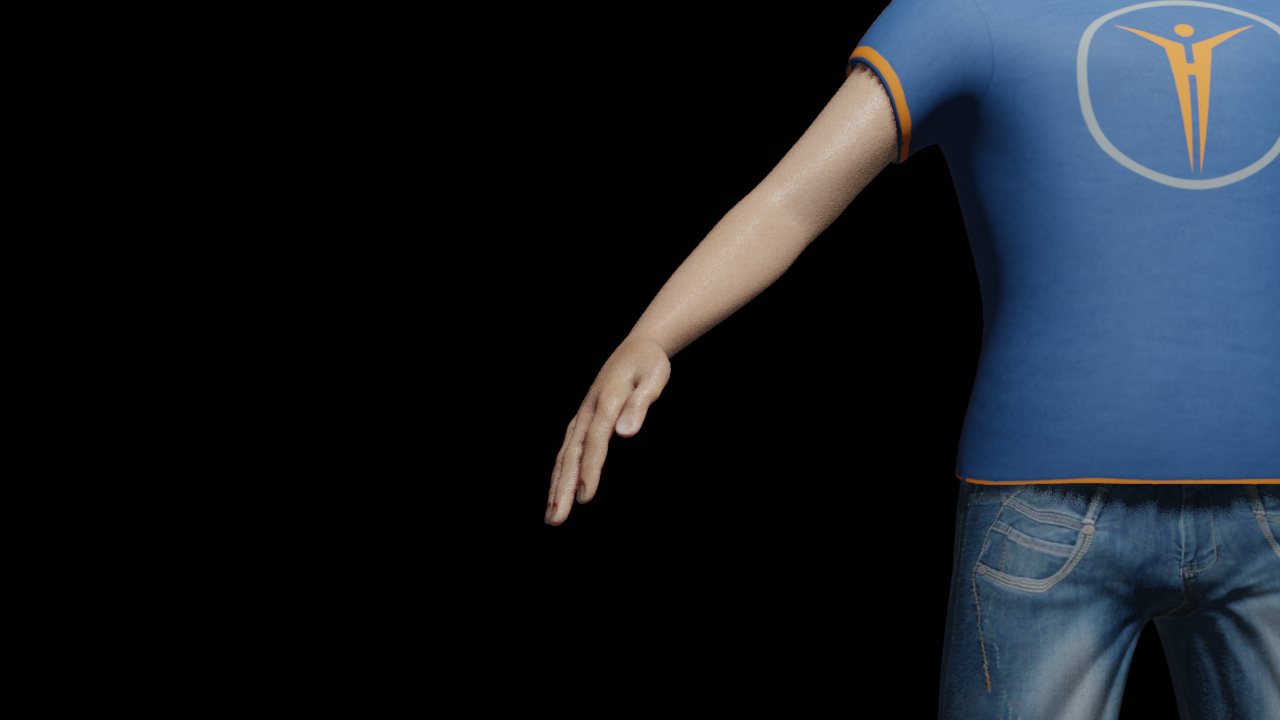
\includegraphics[width=0.1\textwidth]{chapters/avatar_creation_pose_synthesis/images/morph_renders/fingers_spread_R_morph.png} \\

        % Shoulder Morphs
        \texttt{shoulder\_raise\_L} & 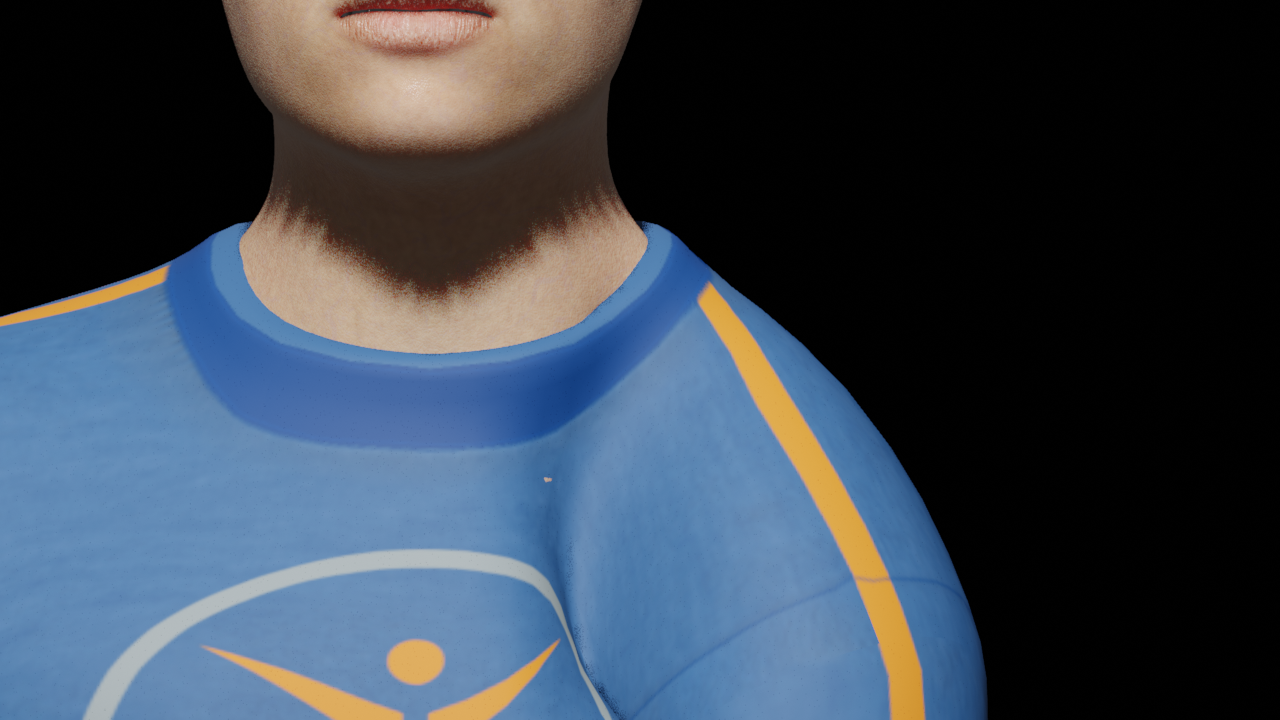
\includegraphics[width=0.1\textwidth]{chapters/avatar_creation_pose_synthesis/images/morph_renders/shoulder_raise_L_morph.png} &
        \texttt{shoulder\_raise\_R} & 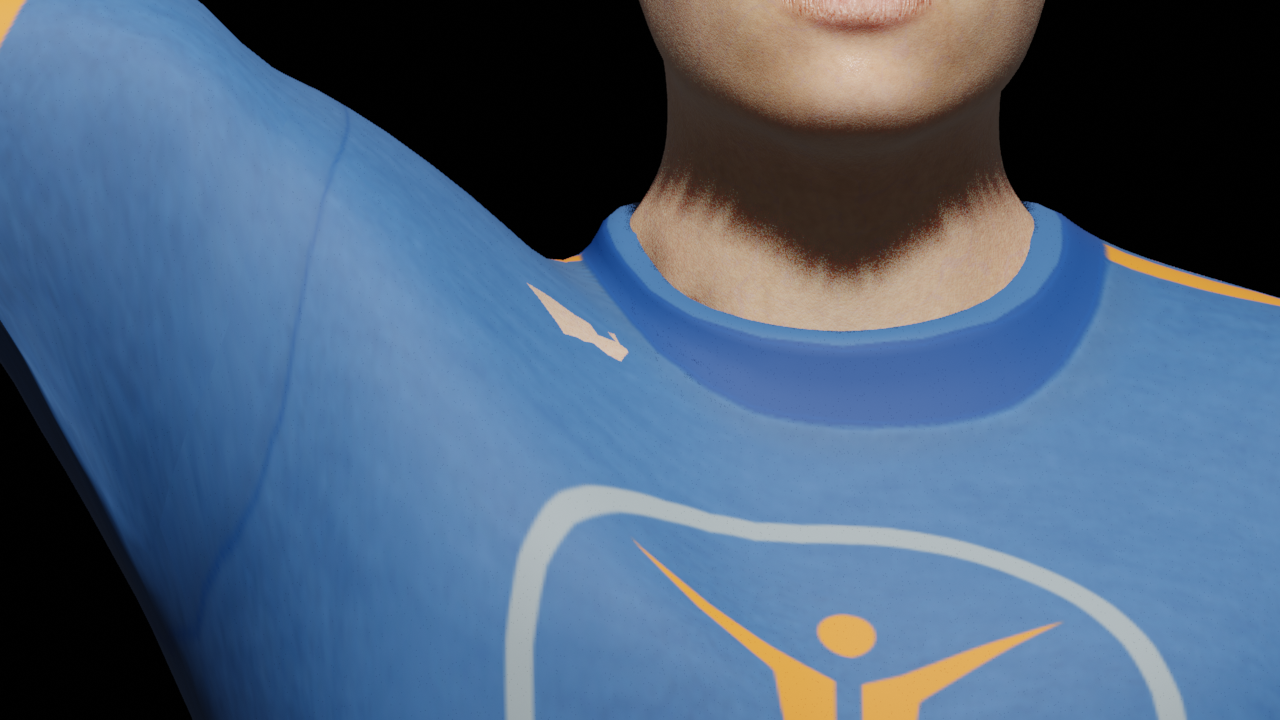
\includegraphics[width=0.1\textwidth]{chapters/avatar_creation_pose_synthesis/images/morph_renders/shoulder_raise_R_morph.png} \\

        \texttt{shoulder\_shrug\_L} & 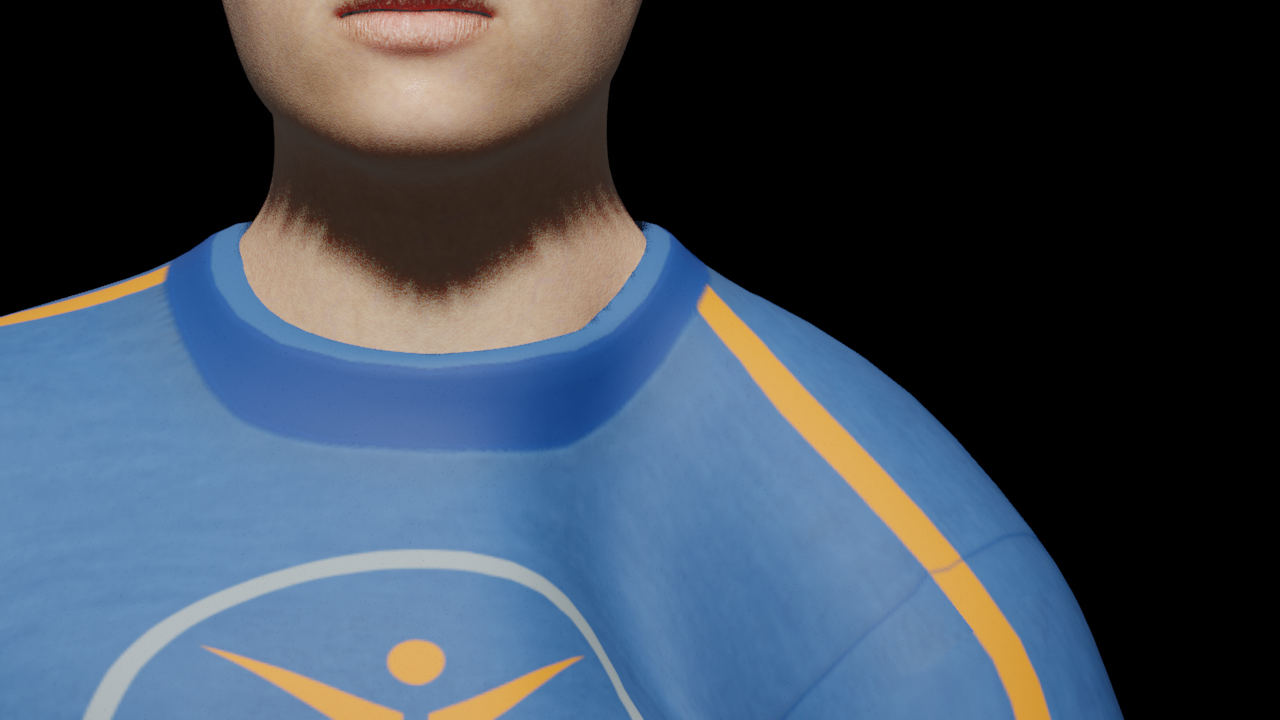
\includegraphics[width=0.1\textwidth]{chapters/avatar_creation_pose_synthesis/images/morph_renders/shoulder_shrug_L_morph.png} &
        \texttt{shoulder\_shrug\_R} & 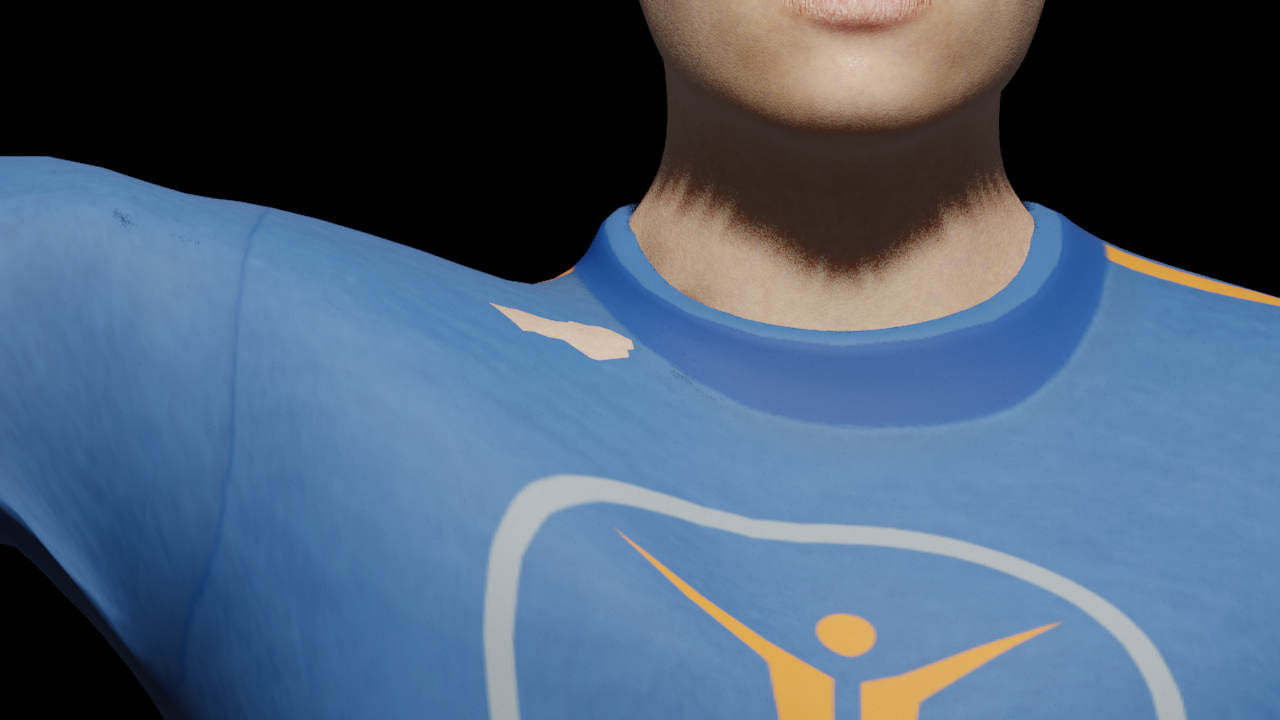
\includegraphics[width=0.1\textwidth]{chapters/avatar_creation_pose_synthesis/images/morph_renders/shoulder_shrug_R_morph.png} \\

        \hline
        % Spine extended spanning both columns and centered
        \multicolumn{2}{|c|}{\texttt{spine\_extended}} &
        \multicolumn{2}{c|}{\centering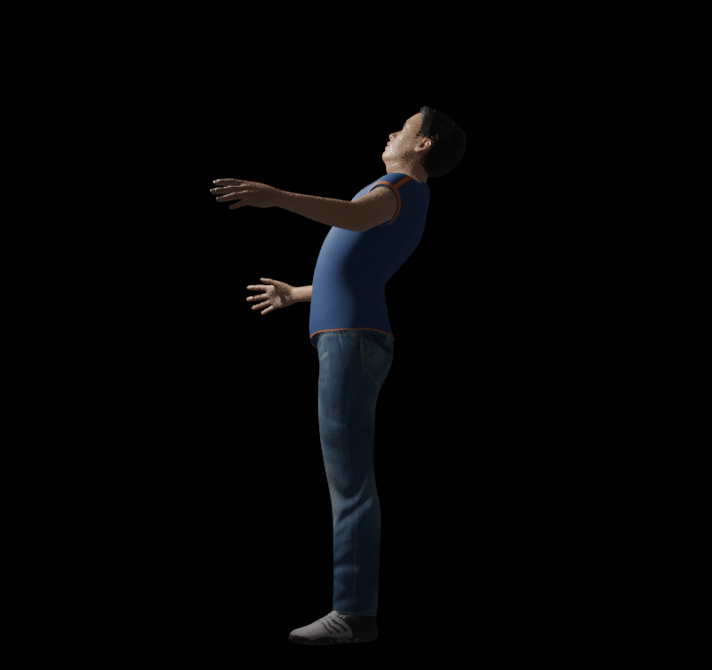
\includegraphics[width=0.25\textwidth]{chapters/avatar_creation_pose_synthesis/images/morph_renders/spine_extended_morph.png}} \\
        \hline
    \end{tabular}
    \caption{Table of skeletal morphs and their effects}
    \label{fig:skeletal_morphs}
\end{figure}


\subsubsection{Facial Morphs}
\label{ch:avatar_creation_pose_synthesis:proc_rig_signing_avatars:morph_constraints:facial_morphs}

Facial morphs in the AZee framework provide a means to represent the complex and nuanced expressions essential for conveying emotions and grammatical cues using subtle facial movements that are integral to effective communication in \gls{sl} (figure~\ref{fig:facial_example}).

\begin{figure}
    \centering
    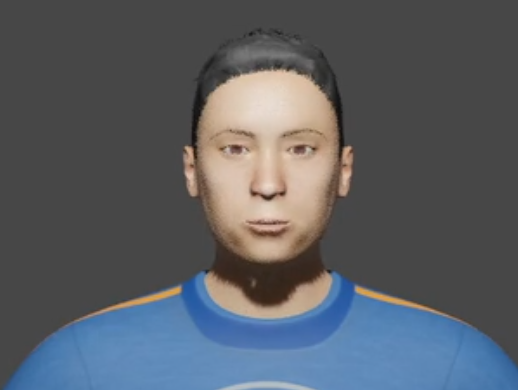
\includegraphics[width=0.5\textwidth]{chapters/avatar_creation_pose_synthesis/images/facial_example.png}
    \caption{Facial morph for \emph{:inter-subjecitivty}}
    \label{fig:facial_example}
\end{figure}

Facial Morph targets are typically generated by sculpting the avatar's mesh into various shapes that correspond to different expressions or gestures. These sculpted shapes are then saved as "keys," which can be blended together during animation to produce the desired expression. This process allows for a high degree of flexibility in animation, as different keys can be combined in real-time to create a wide range of expressions. While this section offers a brief overview, the detailed modeling, implementation, and challenges associated with facial morphs are discussed extensively in Chapter~\ref{ch:facial_expressions}.

\subsubsection{Integration with other layers}
\label{ch:avatar_creation_pose_synthesis:proc_rig_signing_avatars:morph_constraints:intergation}

The morph constraints are integrated along with the other constraints in the posture optimization algorithm. Top optimize skeletal morph constraints we calculate the \gls{fk} values of the impacted bones for skeletal morphs and calculate the loss using rotation distance formula.

\[
d_R = \min\left( 2 \cos^{-1}\left( \left| q_1 \cdot q_2 \right| \right), 2\pi - 2 \cos^{-1}\left( \left| q_1 \cdot q_2 \right| \right) \right)
\]

Where:
\begin{itemize}
    \item \( q_1 \) and \( q_2 \) are the quaternions representing the current and target bone rotations, respectively.
    \item \( q_1 \cdot q_2 \) is the dot product of the two quaternions.
    \item \( \cos^{-1} \) is the inverse cosine function.
    \item The absolute value \( | q_1 \cdot q_2 | \) ensures the angle is within the correct range (0 to \( \pi \)).
    \item The \( \min \) ensures we take the shortest rotation distance.
\end{itemize}

For the the facial morphs however, the morphs act on the mesh and the loss is calculated using the distance between the vertices.

\[
d_V = \frac{1}{N} \sum_{i=1}^{N} \| \mathbf{v}_i - \mathbf{v}_i' \|
\]

Where:
\begin{itemize}
    \item \( N \) is the number of vertices impacted by the morph.
    \item \( \mathbf{v}_i \) is the position of the \( i \)-th vertex in the original mesh.
    \item \( \mathbf{v}_i' \) is the position of the \( i \)-th vertex in the morphed mesh.
    \item \( \|\cdot\| \) denotes the Euclidean distance between corresponding vertices.
\end{itemize}

\section{Results and Implementation}
\label{ch:avatar_creation_pose_synthesis:results}

The layered rigging system has been implemented and tested on the BAZeel (MakeHuman) avatar in blender. The final avatar with layers as well as sites can be seen in figure~\ref{fig:layers_example}.

\begin{figure}
    \centering
    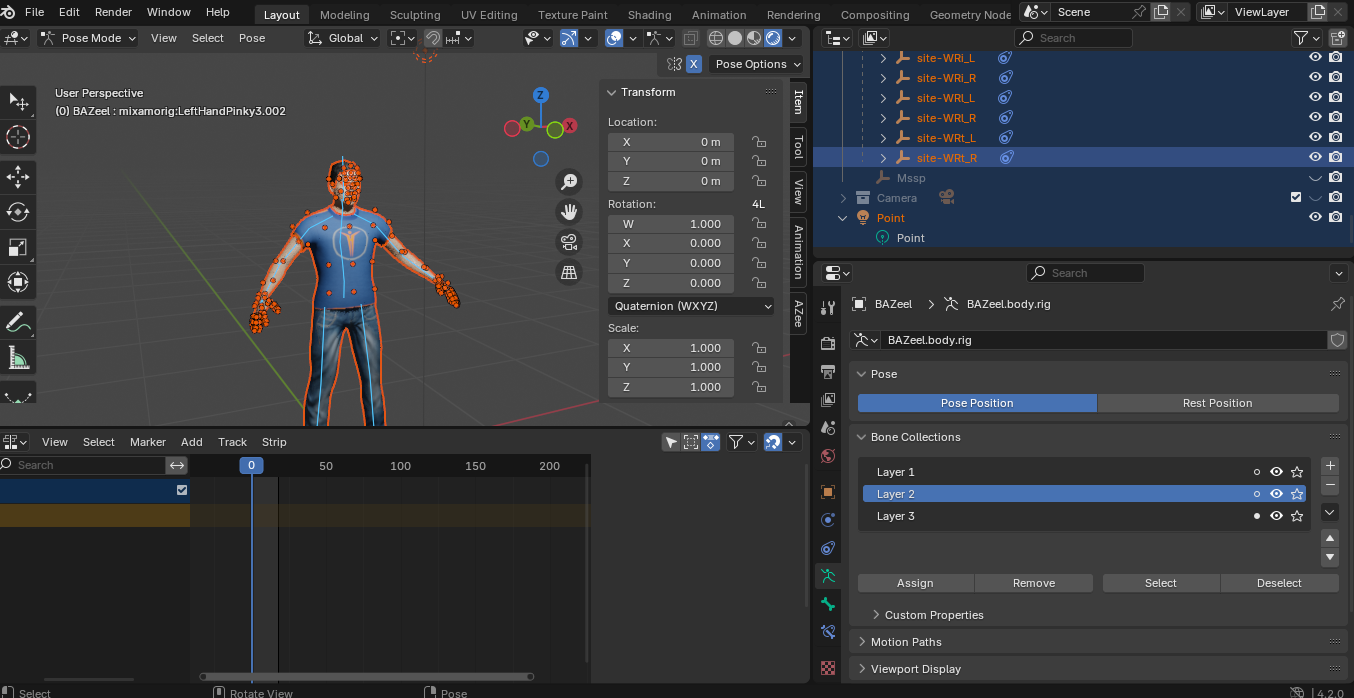
\includegraphics[width=0.5\textwidth]{chapters/avatar_creation_pose_synthesis/images/layers_example.png}
    \caption{Example of the layered rigging system on the BAZeel avatar}
    \label{fig:layers_example}
\end{figure}

The animator is developed as an add-on for blender (see appendix section~\ref{app:avatar_creation_pose_synthesis:animator_class_diagram} for the design diagram) and uses the AZee interpreter as a package to parse the AZee descriptions. The BAZeel avatar was developed using the MakeHuman tool with the default Mixamo rig. 

\section{Evaluation}
\label{ch:avatar_creation_pose_synthesis:evaluation}

We evaluate the quality and the performance of the animation generated by the layered rigging system.

\subsection{Quality of Animation}
\label{ch:avatar_creation_pose_synthesis:evaluation:quality}

The quality of our animations is directly influenced by the AZee descriptions used. Since AZee descriptions can vary in quality, this work will focus solely on whether the constraints specified by the descriptions are satisfied in the resulting animations, without evaluating the quality of the descriptions themselves.

For our tests, the configuration for the posture optimization algorithm were as follows:
\begin{itemize}
    \item Iterations: 20
    \item Distance threshold: 0.1
    \item Rotation threshold: 5 degrees
    \item Solver: \gls{itasc}
\end{itemize}

Video\footnote{\url(www.phd.paritosh-sharma.com/dissertation/ch3comparison.mp4)} shows some \gls{lsf} signs generated by the old and the new synthesizer. The newer system demonstrates improved constraint satisfaction, especially for the sign \emph{:mercredi} (\gls{lsf} for "Wednesday"), using the same posture optimization configuration.

Despite both systems meeting the AZee constraints, the resulting animations remain somewhat robotic and lack the natural fluidity of expressive \gls{sl} gestures. This is because our system solely utilizes the low-level constraint optimization for keyframing the avatar. However, since anything annotated with AZee can be synthesized by our system, this provides a strong foundation for \gls{sl} animation.

\subsection{Performance}
\label{ch:avatar_creation_pose_synthesis:evaluation:performance}

The synthesis time of our newer system compared to the previous synthesizor for some \gls{lsf} signs are shown in table~\ref{tab:faster_executions}. Note that this not account for the time taken to interpret the AZee descriptions. Thus, the older synthesizor goes from an \emph{Animated Score} to keyframes on the blender armature while the newer system goes from a \emph{Synced Score} to keyframes on the blender armature on a \emph{multi-track} timeline (discussed in more detail in chapter~\ref{ch:multi_track}).

\begin{table}
    \centering
    \begin{tabular}{|c|c|c|}
        \hline
        \textbf{AZee description} & \textbf{Old Synthesizor} & \textbf{New Synthesizor}\\
        \hline
        \emph{:arbre} (tree) & 1.58 & \textbf{0.63} \\
        \emph{:bien} (good) & 2.93 & \textbf{1.03} \\
        \emph{:hier} (yesterday) & 5.8 & \textbf{2.2} \\
        \emph{:armoire} (cupboard) & 21.85 & \textbf{8.6} \\
        \hline
    \end{tabular}
    \caption{Synthesis time (in seconds) for both synthesizors}
    \label{tab:faster_executions}
\end{table}

We conducted our experiments on a machine with the following specifications:
\begin{itemize}
    \item Processor: Intel Xeon 6248R
    \item RAM: 32GB
    \item GPU: NVIDIA GeForce RTX A6000
    \item OS: Windows 10
\end{itemize}

We observe that our newer method for synthesis is significantly faster because of direct integration with Blender. The automatic site generation and rigging also reduce the time taken to set up the avatar for animation.

%\subsection{Accuracy of the Animation}
%\label{ch:avatar_creation_pose_synthesis:evaluation:accuracy}

%The accuracy of the animation can be evaluated using the Frechet gesture distance(todo frobenius distance) %calculated using the generated animation and a reference animation based on the AZee body sites. Table~\ref%%{tab:accuracy_metrics} shows the results of the evaluation.

%\begin{table}
%     \centering
%     \begin{tabular}{|c|c|}%         \hline
%         \textbf{Metric} & \textbf{Value} \\
%         \hline
%         Frechet Gesture Distance & todo \\
%         Old synthesizer & todo \\
%         Paula & todo \\
%         Sgnify & todo \\
%         Mocap(Retargeted) & todo \\
%         \hline
%     \end{tabular}
%     \caption{Evaluation metrics for the accuracy of the animation}
%     \label{tab:accuracy_metrics}
% \end{table}

\section{Conclusion}
\label{ch:avatar_creation_pose_synthesis:conclusion}

In this chapter, we presented our methodology to create the signing avatar which we can animate using the AZee descriptions. We used a popular open-source avatar creation tool MakeHuman to create our avatar. We introduced an automatic site generation and rigging process to significantly reduce the time and effort required to set up an avatar for \gls{sl} animation. We also improved the link between AZee's abstract skeleton representation and blender's armature by interfacing them directly with each other. Also, we observed that by dividing the rig into distinct layers, each responsible for a different aspect of the avatar's movement and deformation, we have a more efficient system. Lastly, we observe that our constraint-based posture optimization algorithm is more accurate as well as faster than the previous synthesizer.

However, the animations generated by the system are still robotic and lack the fluidity and expressiveness of natural \gls{sl} gestures. The future work includes improving the quality of the animations, integrating facial expressions, and explores the use of machine learning techniques to enhance the realism and expressiveness of the synthesized discourse.

\end{document}